% This is LLNCS.DEM the demonstration file of
% the LaTeX macro package from Springer-Verlag
% for Lecture Notes in Computer Science,
% version 2.4 for LaTeX2e as of 16. April 2010
%
\documentclass{llncs}
%
%\usepackage{makeidx}  % allows for indexgeneration
\usepackage{wrapfig}
\usepackage{float}
\usepackage[english]{babel}
\usepackage{lipsum}
\usepackage{caption}
\usepackage{subcaption}
\usepackage{graphicx}
	\graphicspath{{images/}} 
%\usepackage{cite}
\usepackage[linesnumbered,ruled]{algorithm2e}
\usepackage{courier}
\usepackage{hyperref}
    \hypersetup{colorlinks=true,allcolors=blue}
\usepackage{listings}
	\lstset{
  		basicstyle=\ttfamily,
  		frame=none, 
  		breaklines=true,
  		numbers=left,
  		xleftmargin=2.5em,
  		framexleftmargin=0em,
    	emphstyle=\textbf,
    	float=t
	}
	\lstdefinestyle{ocl}{
  		emph={
        	context, inv
    	}
	}
	\lstdefinestyle{cbp}{
	    basicstyle=\ttfamily\scriptsize,
  		emph={
        	session, create, of, type,
        	set, to, add, hire
    	}
	}
	\lstdefinestyle{xmi}{
		basicstyle=\ttfamily\scriptsize,
  		emph={
        	Node, children
    	}
	}
	\lstdefinestyle{xml}{
	    basicstyle=\ttfamily\scriptsize,
  		emph={
        	register, create, add, to, resource,
        	from, eattribute, remove, ereference,
        	set, unset, session, Roy, Jen,
        	Moss, Richmond
    	}
	}
	\lstdefinestyle{java}{
	    basicstyle=\ttfamily\scriptsize,
  		emph={
        	case, UNSET,
        	instanceof, else, if, void,
        	new, UnsetEAttributeEvent,
        	UnsetEReferenceEvent,
        	@override, public, class, extends
    	}
	}
	\lstdefinestyle{eol}{
	    basicstyle=\ttfamily\scriptsize,
  		emph={
        	var, new, for, in, create, set, of, with, 
        	unset, to, add, remove, delete, register,
        	from, position, from, move-within, session, \.
    	}
	}

\begin{document}
\renewcommand{\thelstlisting}{\arabic{lstlisting}}
\renewcommand{\labelitemi}{$\bullet$}
\newcommand{\dk}[1]{\textbf{[DK: #1]}}

\title{An Algorithm for Efficient Loading \\ of Change-Based Models}
%
%\titlerunning{Change-based Persistence and Its Loading Optimisation}  % abbreviated title (for running head)
%                                     also used for the TOC unless
%                                     \toctitle is used
%
\author{
    Anonym%Alfa Yohannis \and Horacio Hoyos Rodriguez \and Fiona Polack \and Dimitris Kolovos
}
%
\authorrunning{
    Anonym%Alfa Yohannis et al.
} % abbreviated author list (for running head)
%
%%%% list of authors for the TOC (use if author list has to be modified)
%\tocauthor{Alfa Yohannis,Horacio Hoyos Rodriguez, Fiona Polack, Dimitris Kolovos}
%

\institute{anonym}
%\institute{Department of Computer Science, University of York, United Kingdom\\
%\email{\{ary506, horacio.hoyos, dimitris.kolovos, fiona.polack\}@york.ac.uk}}

\maketitle              % typeset the title of the contribution
%The first states the problem. The second states why the problem is a problem. The third is my startling sentence. The fourth states the implication of my startling sentence.
\begin{abstract}
% The benefits obtained from using changed-based persistence (CBP) for object-oriented (MOF/Ecore) models comes at the cost of increased load costs. The additional cost can outweigh the benefits and as a result CBP may not be widely adopted. By providing an optimized loading mechanism the load times of CBP can be improved. By reducing the load times, CBP will be widely adopted and allow tools to provide better collaborative modelling environments, support faster incremental model validation and transformation, among others. Our results show show that the proposed optimizations can improve loading times up to 80\% compared to the original CBP; further, the results show improved store performance against the existing CBP solution while preserving constant store times.

Recent work proposed a language-independent change-based persistence (CBP) approach for models conforming to object-oriented metamodelling architectures such as MOF and EMF. In this approach, instead of persisting the state of a model, its full editing history is persisted, and the state of the model is reconstructed at loading time by replaying this history. Storing the entire editing history is beneficial for precise change detection -- and hence e.g. model merging, incremental execution of model management programs -- but comes at the cost of larger and ever-growing model files and slower loading. In this paper, we contribute a more efficient algorithm for loading models stored in a change-based format. The proposed algorithm identifies and skips changes that are superseded by latter changes -- and which therefore have no impact on the eventual state of the model. We evaluate the performance of the new loading algorithm experimentally and we assess the impact it has on saving change-based models. Our results show that the proposed algorithm can reduce loading times by up to 44\% compared to the naive CBP loading algorithm, with a negligible impact on saving.

\end{abstract}

\section{Introduction}
\label{sec:introduction}
Existing approaches for file-based persistence of models in metamodelling architectures such as MOF and EMF are predominately state-based.
In such approaches, model files contain snapshots of the models' contents, and activities such as version control and change detection are left to external systems such as file-based version-control systems and model differencing facilities.
Activities such as model comparison and change detection are computationally consuming for state-based models and can become a burden as larger models are developed in a collaborative setting. 

In contrast to persisting the \emph{state} of models, we harness a change-based approach that persists the full sequence of \emph{changes} made to models instead.
The change-based approach comes with a number of envisioned benefits over stated-based persistence, such as the ability to detect changes much faster and more precisely\,\cite{yohannis2017turning}, which can then have positive knock-on effects on helping developers to diff/merge models in collaborative modelling environments, as well as on facilitating faster incremental model validation and transformation\,\cite{rath2012derived,ogunyomi2015property}.
However, change-based persistence comes at the cost of larger and ever-growing model files, and increased model loading time since all recorded changes need to be replayed to reconstruct a model's state\,\cite{yohannis2017turning}.   

Our work extends the work of Yohannis et al. \cite{yohannis2017turning} that implements a change-based persistence (CBP) format, and proposes and evaluates an algorithm that reduces loading time of change-based models by avoiding replaying changes that have no impact on the eventual state of the model (e.g. that are superseded by subsequent changes).
% We assess the efficiency of the algorithm in terms of loading and persistence time, and memory footprint.
% Our approach demonstrates considerable savings in loading times when compared to the previous work, while the effects on the store time are negligible. %\dk{If the contribution we're proposing in this paper is the optimised loading algorithm, starting that loading cost is higher can be confusing.}%\hh{This this was copied form the previous paper, so fixed now.}

The rest of the paper is structured as follows. Section \ref{sec:case_study} introduces a running example and provides a brief overview of the original change-based model persistence approach.
Section \ref{sec:loading_time_optimisation} presents an algorithm that intends to speed up loading of change-based models, and its supporting data structures. %\dk{Merge Sections 3 and 4}.  
Sect. \ref{sec:performance_evaluation} discusses the results of controlled evaluation experiments for assessing the benefits of the proposed algorithm. Section \ref{sec:related_work} provides an overview of related work, and Sect. \ref{sec:conclusions} concludes this paper and discusses directions for future work.

\section{Running Example}
\label{sec:case_study}
To explain change-based model persistence and the contribution of this work, we use the minimal tree metamodel (expressed in the Eclipse Modelling Framework's Ecore metamodelling language) and model illustrated in Figures \ref{fig:tree_metamodel} and \ref{fig:initial_model}.
We chose EMF/Ecore as the de-facto standard in object-oriented metamodelling, and this contrived example to avoid superseded repetition in our discussion, while providing a reasonable coverage of the core features of Ecore (classes, single/multi-valued features, references and attributes).
In this example, tree models consist of named nodes which can -- optionally -- contain other nodes (\emph{children} reference).

\begin{figure}[ht]
    \begin{subfigure}[t]{0.4\linewidth}
        \centering
        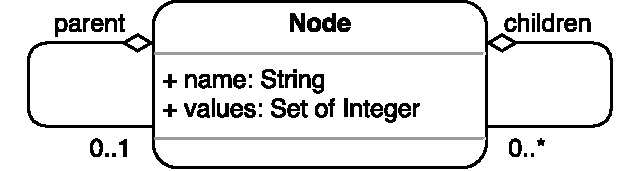
\includegraphics[width=0.8\linewidth]{node_metamodel}
        \caption{The tree metamodel.}
        \label{fig:tree_metamodel}
    \end{subfigure}
    \hfill
    \begin{subfigure}[t]{0.6\linewidth}
        \centering
        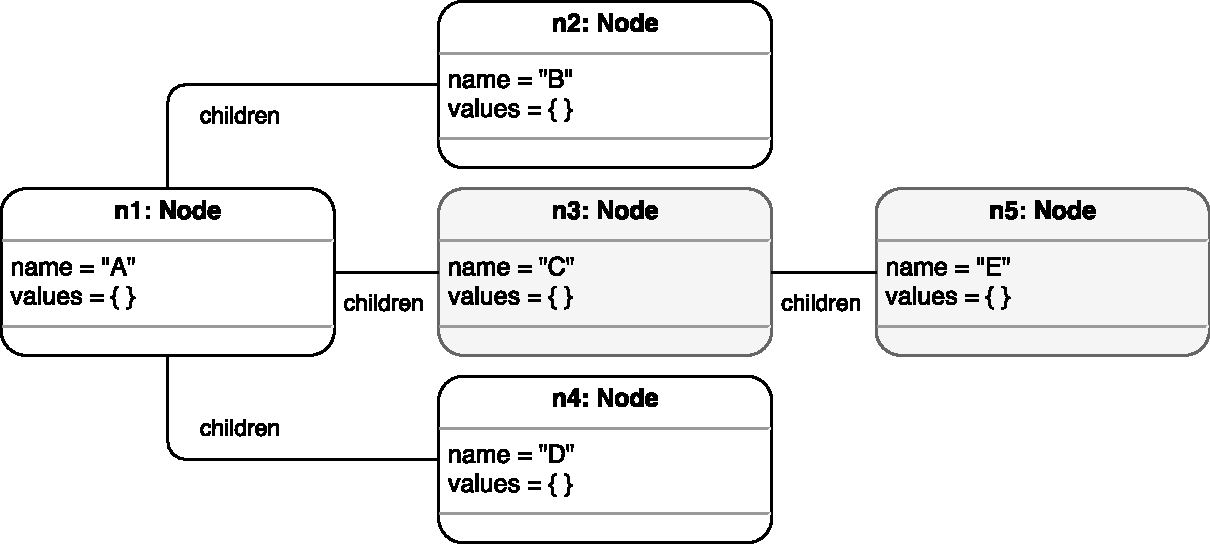
\includegraphics[width=0.6\linewidth]{initial_chart}
        \caption{A model that conforms to the tree metamodel (n3 was created and then deleted)}
        \label{fig:initial_model}
    \end{subfigure}
    \caption{A tree metamodel and its model as the running example.}
    \label{fig:append_speed}
\end{figure}

The model in Fig. \ref{fig:initial_model} consists of two nodes \emph{n1}, \emph{n2}.
To construct this model, we started by creating and naming three nodes (\emph{n1}, \emph{n2} and \emph{n3}).
Nodes \emph{n2} and \emph{n3} were then added as children of \emph{n1}.
Finally, node \emph{n3} was deleted from the model.
The final state of the model is presented in a simplified (state-based) XMI representation in Listing \ref{lst:xmimodel}.

\noindent
\begin{minipage}[t]{0.34\linewidth}
\begin{lstlisting}[style=xmi,caption={State-based representation of the tree model in (simplified) XMI.},label=lst:xmimodel]
<Node id="n1" name="A">
  <children id="n2" 
    name="B"/>
</Node>
\end{lstlisting}
\end{minipage}
\hfill
\begin{minipage}[t]{0.635\linewidth}
\begin{lstlisting}[style=eol,caption={Change-based representation of the tree model.},label=lst:cbpmodel]
create n1 of Node
set n1.name to "A"      
create n2 of Node
set n2.name to "B"      
create n3 of Node
set n3.name to "C"      
add n2 to n1.children   
add n3 to n1.children
remove n3 from n1.children   
delete n3
\end{lstlisting}
\end{minipage}

In contrast to the state-based representation, a CBP representation of the model is illustrated in Listing \ref{lst:cbpmodel} (the syntax is a simplified version of the one introduced in\,\cite{yohannis2017turning}).
Lines 1-6 record the creation and naming of the three nodes, lines 7 and 8 record the addition of \emph{n2} and \emph{n3} as children of \emph{n1} and lines 9-10 capture the deletion of \emph{n3} (deletion effectively involves two events).

% Instead of treating the model as a state based, we records all events generated by the the consecutive  operations and persist them into a CBP representation (Listing \ref{lst:cbpmodel}), which contains at least as much information as the state-based representation. Replaying all these events produces the same state as the one captured in the Listing \ref{lst:xmimodel}.  

For small changes made to large models, this approach can be beneficial since we only need to persist the change events every time -- as opposed to the entire model.
However, loading the model by naively replaying all the events,\cite{yohannis2017turning} is not optimal particularly for models with long editing histories where prior events are effectively superseded by subsequent events. For example, creating \emph{n3} in line 5, naming it in line 6, and adding it to the children of \emph{n1} in line 8 are cancelled by the subsequent deletion of \emph{n3} in line 10. As such, the events in lines 5, 6, 8, 9 and 10 could be ignored during the loading process without affecting the eventual state of the model.

%An optimisation can be performed by ignoring the superseded events. For example, the deletion of node \emph{n3} makes events (Listing \ref{lst:xmimodel}, lines 5-6, 8-10) related to the node superseded to be replayed. 

\section{Towards Efficient Loading of Change-Based Models}
\label{sec:loading_time_optimisation}
The flowchart in Fig. \ref{fig:flowchart} provides an overview of the editing lifecycle of a model under the proposed approach, and the different artefacts involved in it. It also highlights (starred blocks) the extensions proposed compared to the original CBP approach in \cite{yohannis2017turning}.

In the original CBP approach in \cite{yohannis2017turning}, a modelling session involves three activities: loading a model, editing it, and saving changes back to the model file. After saving a model, the user can make further edits and save them again. Loading is achieved by reading and replaying a sequence of change events stored in a CBP-formatted file. During the editing process, changes to the model are stored in a memory-based data structure (``Change events''), which are serialised and appended at the end of the CBP-formatted model file, and then flushed from memory, every time the model is saved.

The proposed approach adds two new artefacts: a ``Model History'' data structure which is populated with change events and which is used to detect superseded events prior to saving, and an ``Ignore List'' file for each CBP model, which persists the position (i.e. line numbers) of superseded events so that they can be ignored the next time the model is loaded.

% In constructing a model, an agent (i.e. person, software program) initially starts by loading an empty model. The agent then proceeds to edit the model by executing a range of operations (create, add, remove, etc.). Events generated by performing these operations are collected and stored into a list of change events in memory. 

\begin{figure}[ht]
\centering
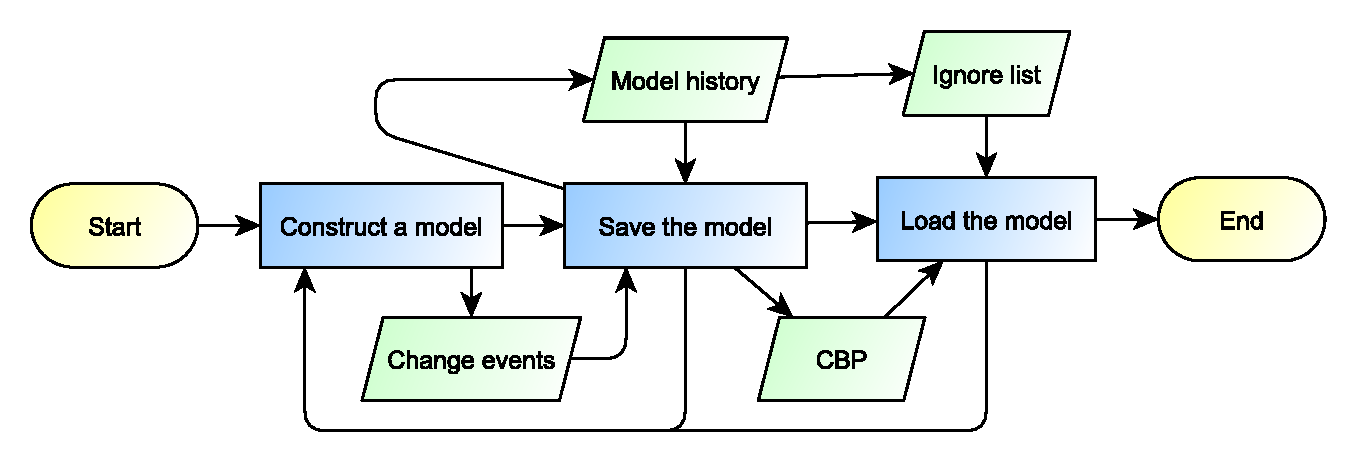
\includegraphics[width=\linewidth]{flowchart}
\caption{The context flowchart of optimising loading performance of CBP.}
\label{fig:flowchart}
\end{figure}

% After some time working on the model, the agent needs to save the model.
% Instead of saving the last state of the model, the CBP implementation persists the change events.
% The saving activity produces three types of data: a Model History, an Ignore List, and a CBP model.
% The Model History and Ignore List are additional to the original CBP implementation.
% The Model History is populated when our implementation by iterating over the change events.
% Elements, features, event types, lines, and values involved in each of the events are stored into the Model History.
% After populating the Model History, the proposed algorithm is executed to identify events that are superseded and they are stored in the Ignore List.
% After that, the Ignore List is persisted. 
% 
% Some time later the agent decides to reload the model persisted in the CBP format.
% In the loading activity, the Ignore List is loaded first before loading the model.
% The events contained in the Ignore List are used as references to check whether an event in the CBP model is ignored for replay or not, thus reducing the effective number of events that are replayed events.   

\subsection{Model History}
\label{subsec:model_history}
The proposed algorithm uses a data structure that memorises elements' events and their position (line number) in a CBP representation so it can reason about the events of a particular element and determine which of them are superseded.
For the rest of the discussion the line number in the CBP representation is referred to as the \emph{event number}.
The proposed data structure is presented in Fig. \ref{fig:object_history} as a class diagram.  

%THE EVENT HISTORY SHOULD ONLY HAVE ONE Line
%ElementHistory HAS THE IsMoved FLAG BUT THE ALGORITHMS USE THE isFeatureMoved... why?

\begin{figure}[ht]
\centering
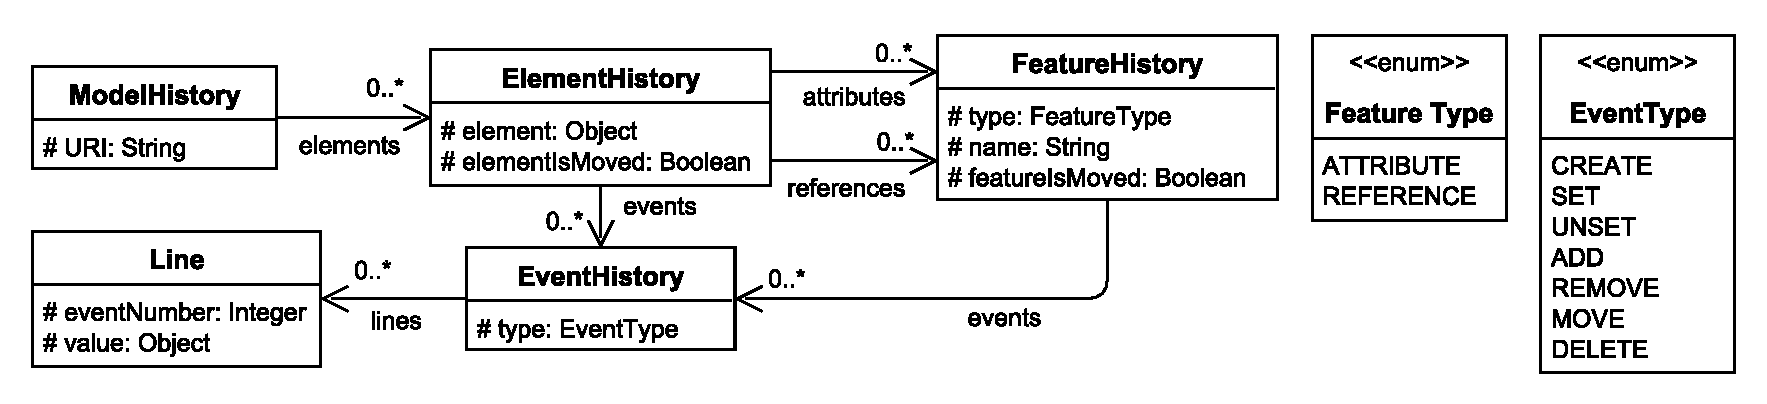
\includegraphics[width=\linewidth]{object_history}
\caption{The class diagram of Model History.}
\label{fig:object_history}
\end{figure}

\begin{figure}[ht]
\centering
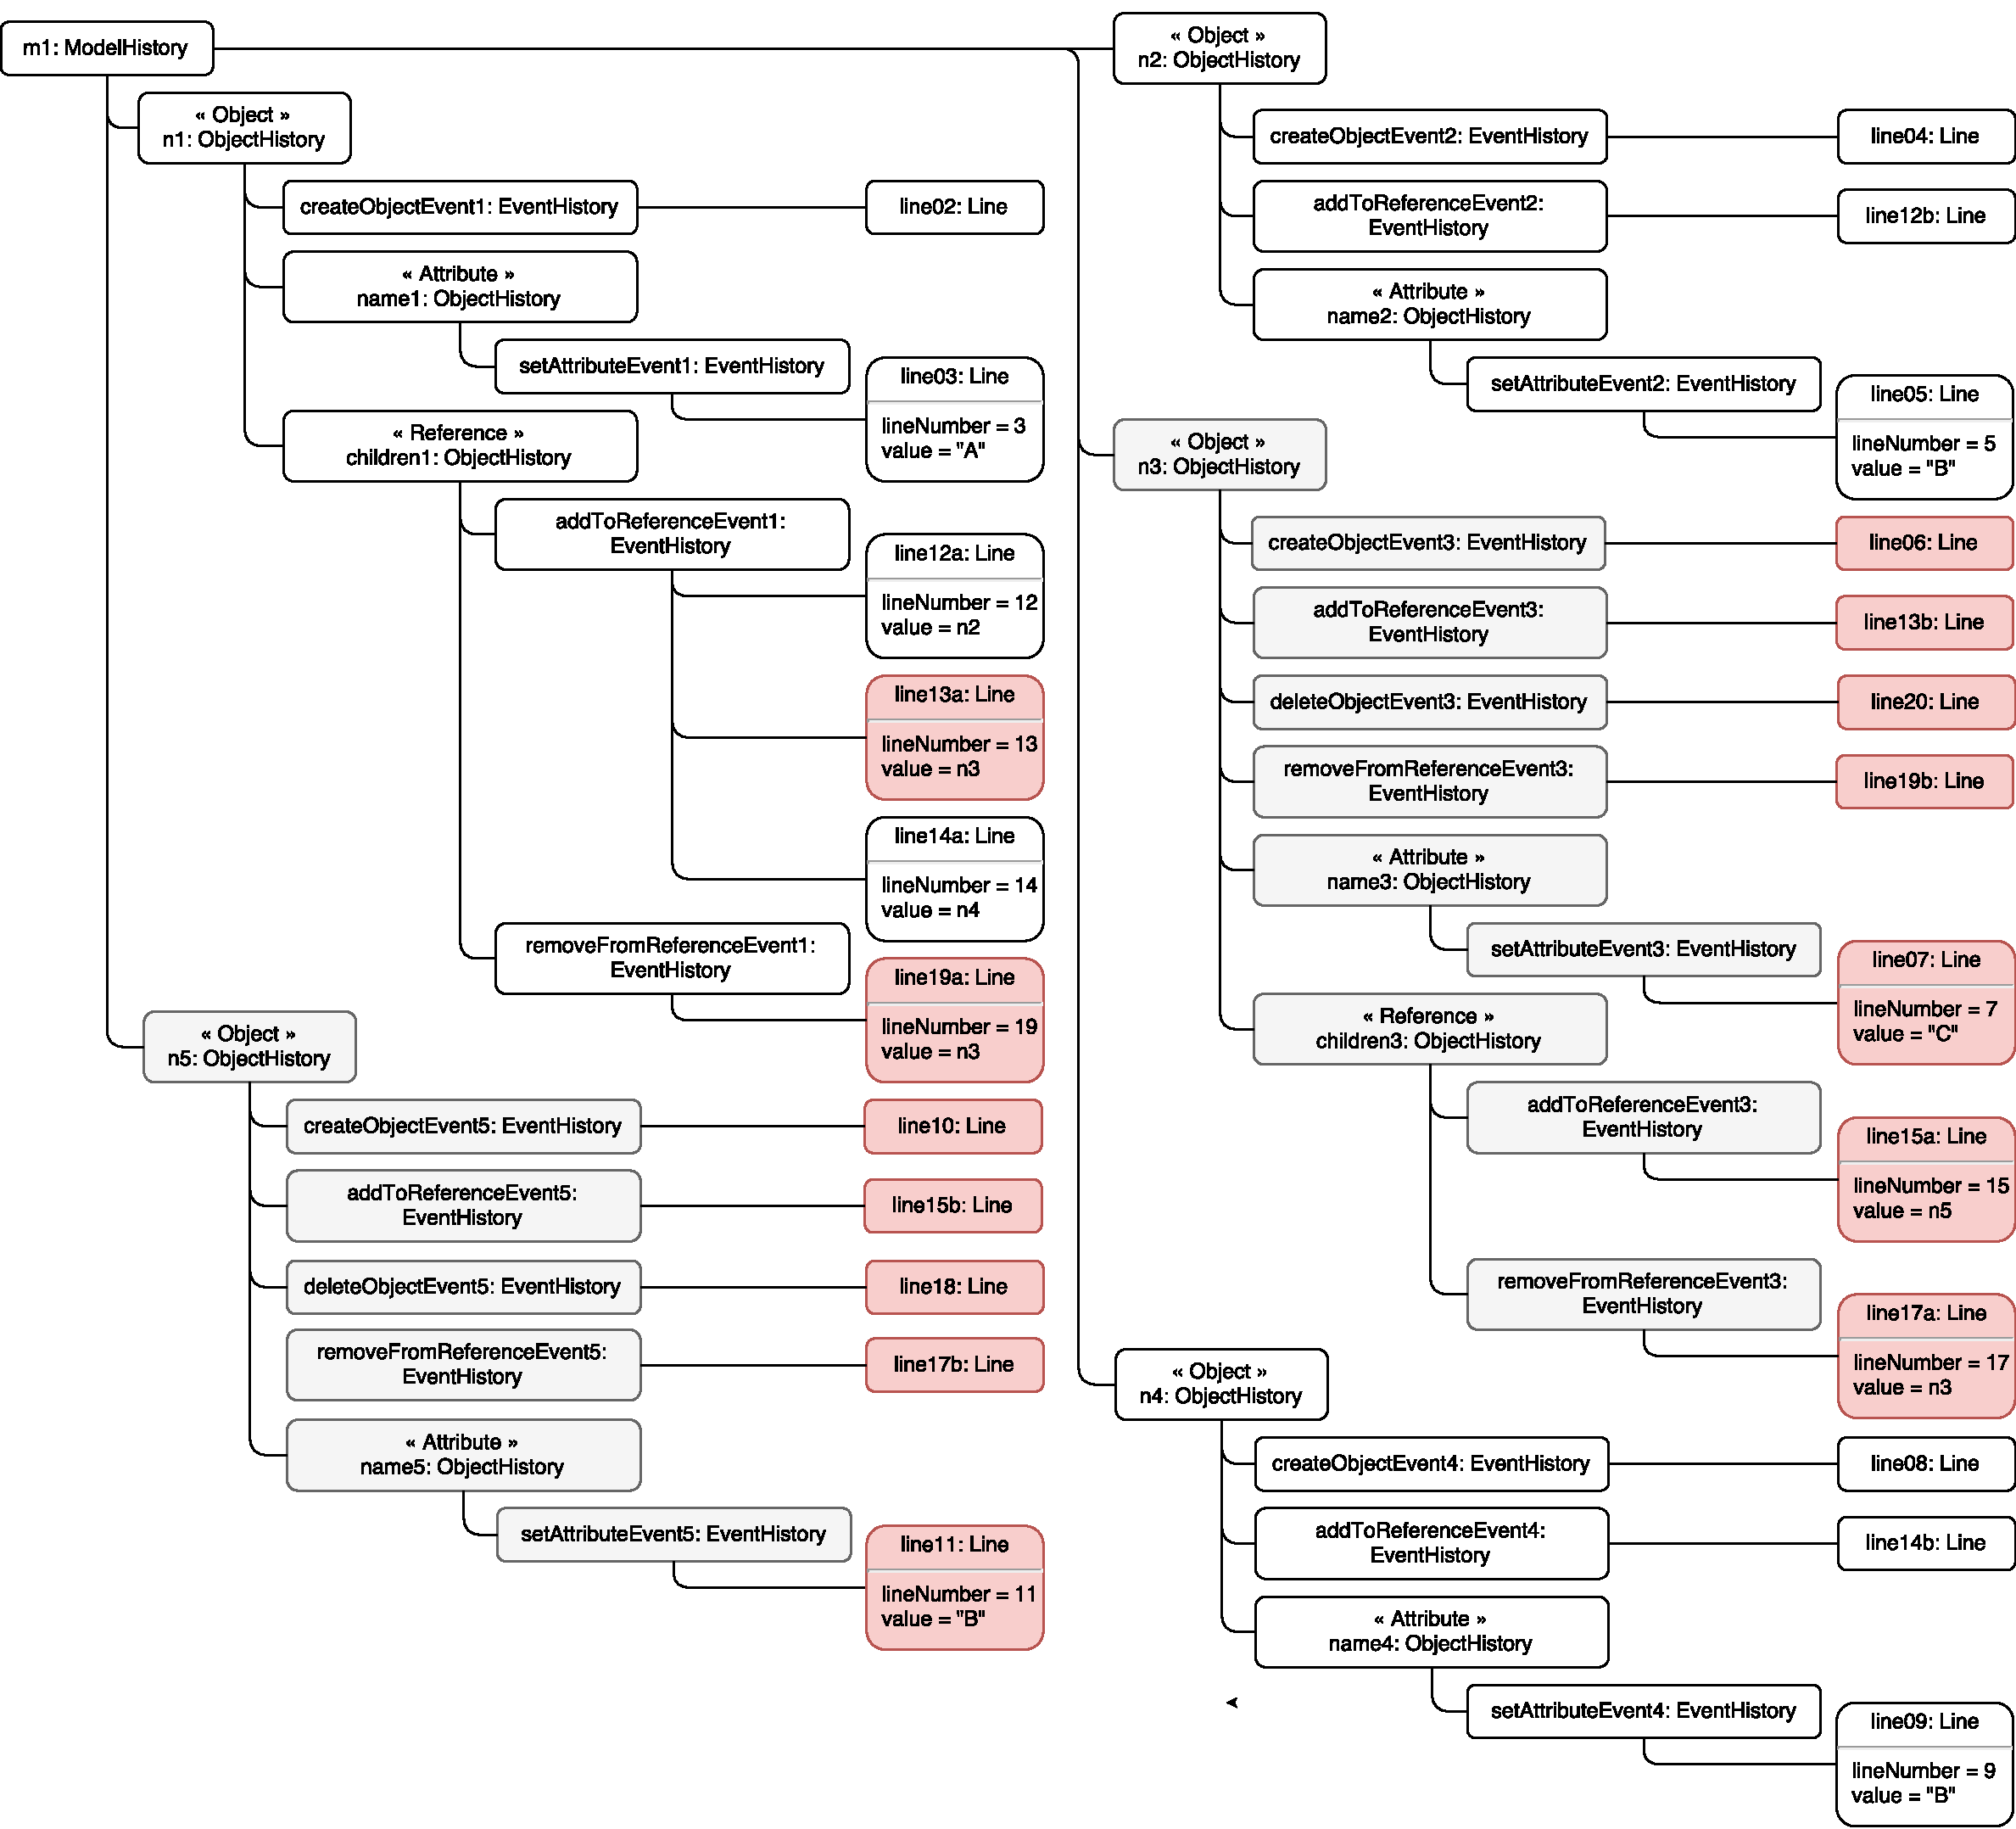
\includegraphics[width=\linewidth]{history_structure}
\caption{The object diagram of the model history of the CBP model in Listing \ref{lst:cbpmodel}.}
\label{fig:history_structure}
\end{figure}

A \emph{ModelHistory} has a \emph{URI} attribute to identify the model for which it records changes and can have many \emph{ElementHistory} elements.
An \emph{ElementHistory} has an \emph{element} field that identifies the element that it refers to and an \emph{elementIsMoved} boolean flag. The  \emph{elementIsMoved} flag is used to indicate a \emph{move} event for the element (section \ref{subsec:add_remove_and_move_operations} provides details of its use).
Every \emph{ElementHistory} can have many \emph{FeatureHistories} to represent the editing histories of individual features (i.e. references/attributes) of the element. 
%that are involved in certain events (i.e. ``\emph{add n2 to n1.children}" event has the \emph{children} as the feature).
A \emph{FeatureHistory} has three fields: \emph{type} to identify its type (attribute or reference), \emph{name} to identify the feature's name, and \emph{featureIsMoved} that has the same role as attribute \emph{elementIsMoved} in \emph{ElementHistory}.

An \emph{EventHistory} represents an event in the CBP model.
An \emph{EventHistory} has an attribute \emph{type} to identify the event's type and can have many \emph{Line}s.
A \emph{Line} has an \emph{eventNumber} attribute to store the line number in the CBP model and a \emph{value} that is used to store the element involved in the event (it is only used for \emph{ADD}, \emph{REMOVE} and \emph{MOVE} events).

Each \emph{FeatureHistory} can have many \emph{EventHistories} to represent the events that modify the value of the feature.
Each \emph{ElementHistory} can have many \emph{EventHistories} to represent events that affect the state of the element (life-cycle and relations to multivalued features).
%For events that involve the element individually (e.g. create, add) element's feature but only affect the element (i.e. ``\emph{create n1 of Node}" event has no feature involved), or events in which an element acts as an operand for a multi-valued feature (i.e. ``\emph{add n3 to n1.children}" event has the \emph{n3} as the operand).
%These kinds of events can have their \emph{EventHistory} belong to their \emph{ElementHistory} directly.

Figure \ref{fig:history_structure} shows the object diagram of the model history of the CBP model in Listing \ref{lst:cbpmodel} (some attribute values are not shown). The grey rectangles are \emph{History} objects that belong to the deleted node \emph{n3}. The  rectangles with the dashed outline are \emph{Line} objects that represent superseded events.

Next, we present the algorithms that use the information stored in the model history data structure to identify events that have no impact in the final state of the model, i.e. superseded events. The algorithms produce the ignore that is used in the proposed CBP loading algorithm.
%WE ARE MISSING SOMETHING THAT SAYS HOW EACH ALGORITHM IS INVOKED FOR EACH FEATURE/ELEMENT AND THAT THE COMPLETE Ignore List IS THE UNION OF ALL IGNORE LSITS?

\subsection{Set and Unset Events}
\label{subsec:set_and_unset_events}
During the lifecycle of a model, a single-valued feature can be assigned many times.
Each of the assignments is persisted as an event in the CBP model.
However, only the last assigned value is necessary to obtain the current state of the feature. 
That is, all events but the last can be ignored.
For example, in Listing \ref{lst:set_unset_example}, the feature \emph{name} is assigned the ``A" value, nullified (unset), and finally assigned the ``B" value.
That is, in the last state of the model: \emph{n1.name = ``B"}.
As a result, the loading process could ignore all previous change events (lines 2 and 3) and only replay the last assignment event (line 4). 

\begin{lstlisting}[style=eol,caption={The CBP representation of attribute \emph{name} assignments.},label=lst:set_unset_example]
create n1 of Node
set n1.name to "A"
unset n1.name
set n1.name to "B"
\end{lstlisting}

%\noindent
%\begin{minipage}[t]{0.49\linewidth}

%\end{minipage}
%\hfill
%\begin{minipage}[t]{0.49\linewidth}
%\begin{lstlisting}[style=eol,caption={The CBP representation of reference  \emph{parent} assignments.},label=lst:set_unset_reference]
%create n1 of Node
%create n2 of Node
%create n3 of Node
%set n3.parent to n1
%set n3.parent to n2
%unset n3.parent
%\end{lstlisting}
%\end{minipage}

The algorithm that identifies superseded \emph{SET} and \emph{UNSET} events for a feature is presented in Alg. \ref{alg:set_unset_optimisation}.
The algorithm has two inputs: a list of event numbers of \emph{SET} events and a list of event numbers of \emph{UNSET} events.
The output of the algorithm is an \emph{ignoreList} that includes the event numbers that are superseded.
The inputs lists can be trivially constructed from the model history data structure.
For the \emph{name} feature in Listing \ref{lst:set_unset_example} these are: $setEventNumbers = \{2,4\}$ and $unsetEventNumbers = \{3\}$.

\begin{algorithm}[H]
\begin{small}
\SetKwInOut{Input}{input}
\SetKwInOut{Output}{output}
\Input{two lists of Integer $setEventNumbers$}
\Output{a list of Integer $ignoreList$}
\SetKwBlock{Beginn}{beginn}{ende}
\Begin{
$setLastLine$ $\leftarrow$ getLastLine($setEventNumbers$)\;
$unsetLastLine$ $\leftarrow$ getLastLine($unsetEventNumbers$)\;
\uIf{$setLastLine > unsetLastLine$}{
    $ignoreList \leftarrow (setEventNumbers \cup unsetEventNumbers) \setminus \{setLastLine\} $\;
}
\ElseIf{$setLastLine < unsetLastLine$}{
    $ignoreList \leftarrow (setEventNumbers \cup unsetEventNumbers)$\;
}
\Return{$ignoreList$}\;
}
\end{small}
\caption{Algorithm to identify event numbers of superseded \emph{set} and \emph{unset} events}
\label{alg:set_unset_optimisation}
\end{algorithm}

The \emph{ignoreList} is populated as follows.
In lines 4 and 5, the last event number of each input list is stored in \emph{setLastLine} and \emph{unsetLastLine} respectively.
If $setLastLine > unsetLastLine$ (line 7) then $ignoreList = (setEventNumbers \cup unsetEventNumbers) \setminus  \{setLastLine\} $, i.e. all events except the last \emph{SET} event can be ignored.
If $setLastLine > unsetLastLine$ (line 9) then $ignoreList = (setEventNumbers \cup unsetEventNumbers)$, i.e. all events can be ignored.
For the \emph{name} feature in Listing \ref{lst:set_unset_example} $ignoreList = \{2, 3\}$.

\subsection{Add, Remove, and Move Events}\label{subsec:add_remove_and_move_operations}
%DO WE SAY HERE THAT THE LIMITATION IS THAT IT ONLY WORKS IN UNIQUE COLLECTIONS?
Similarly, the contents of a multi-valued feature can be modified many times.
If the same element is added and removed multiple times,  only that last event is necessary to determine if the element should appear in the multi-valued feature values in the final state of the feature.
For example, in Listing \ref{lst:add_remove_move_reference},  nodes \emph{n2} and \emph{n3} are added to the \emph{children} feature of \emph{n1} (lines 4-5), and then \emph{n3} is removed (line 6).
That is, in the last state of the model: \emph{n1.children = [n2]}.
As a result, the loading process could ignore the events that represent the \emph{ADD} and \emph{REMOVE} events of \emph{n3}. So far, the algorithm only supports unique features (i.e. features that do not allow duplicate values). An extension to support duplicate values is part of our future work. 

\begin{lstlisting}[style=eol,caption={Example of CBP representation of attribute \emph{values}'s add and remove operations.},label=lst:add_remove_move_reference]
create n1 of Node
create n2 of Node
create n3 of Node
add n2 to n1.children
add n3 to n1.children
remove n3 from n1.children
\end{lstlisting}

\begin{algorithm}[H]
\begin{small}
\SetKwInOut{Input}{input}
\SetKwInOut{Output}{output}
\SetKwProg{Struct}{struct}{}{end}
\Struct{Line}{
    Integer $eventNumber$;
    Anytype $value$;
}
\Input{two lists of Line $addEventLines$, $removeEventLines$, a variable of Anytype $operandValue$, a variable of Boolean $featureIsMoved$} % and $moveEventLines$, , an variable of Feature $feature$}
\Output{a list of Integer $ignoreList$}
\SetKwBlock{Beginn}{beginn}{ende}
\Begin{
\If{$featureIsMoved$ = false}{
    $filteredAddLines$ $\leftarrow$ filterByValue($addEventLines$, $operandValue$)\;
$filteredRemoveLines$ $\leftarrow$ filterByValue($removeEventLines$, $operandValue$)\;
$addLastLine$ $\leftarrow$ getLastLine($filteredAddLines$)\;
$removeLastLine$ $\leftarrow$ getLastLine($filteredRemoveLines$)\;
\uIf{$addLastLine > removeLastLine$}{
     $ignoreList \leftarrow (filteredAddLines.eventNumber \cup filteredRemoveLines.eventNumber \setminus \{addLastLine\} $\;
}
\ElseIf{$addLastLine < removeLastLine$}{
    $ignoreList \leftarrow (filteredAddLines.eventNumber \cup filteredRemoveLines.eventNumber$\;
}
}
%\If{feature is empty}{
%       Add all event numbers in $addEventLines$, $removeEventLines$, and $moveEventLines$ into $ignoreList$\;
%        $attributeIsMoved$ $\leftarrow$ false\;
%}
\Return{$ignoreList$}\;
}
\end{small}
\caption{Algorithm to identify event numbers of superseded \emph{add}, \emph{remove}, and \emph{move} events.}
\label{alg:add_remove_move_optimisation}
\end{algorithm}

%I REMOVED THE "feature is empty" CONDITION BECAUSE IT COMPLICATES THE EXPLANATION AND DOES NOT \emph{ADD} TO THE DISCUSSION. FURTHER, THE UNION OF ALL Ignore ListS WILL BE THE SAME AS THE UNION INSIDE THE CONDITION. 

The algorithm that identifies superseded \emph{ADD} and \emph{REMOVE} events for a feature is presented in Alg. \ref{alg:add_remove_move_optimisation}.
The algorithm has four inputs: a list of Line objects of \emph{ADD} events, a list of Line objects of \emph{REMOVE} events, the element of interest and a flag that indicates a \emph{MOVE} event on the analysed feature. 
The output of the algorithm is an \emph{ignoreList} that includes the event numbers that are superseded.
The inputs lists can be easily constructed from the Model History data structure.
For the \emph{children} feature in Listing \ref{lst:add_remove_move_reference} these are: $addEventLines = \{  \{4, n2 \}, \{5, n3 \} \}$, $removeEventLines = \{\{6, n3 \}\}$, $moveEventLines = \emptyset$,\linebreak $operandValue = n3$, and $featureIsMoved = \mathrm{False}$

The \emph{ignoreList} is populated as follows.
If the flag \emph{featureIsMoved} is true then nothing is added to the list (the need for this flag is explained later in this section).
If the flag \emph{featureIsMoved} is false, then lines 6 and 7 filter the $addEventLines$ and $removeEventLines$ to only keep Lines for which the \emph{value} is equal to \emph{operandValue}.
The filtered lists are stored in $filteredAddLines$ and $filteredRemoveLines$ respectively.
The rest of the algorithm works similar to Alg. \ref{alg:set_unset_optimisation}, ignoring all events but the last if it was an \emph{ADD}, else ignoring all events. 

%However, this logics can only be executed if there is no \emph{move} event has been applied to the feature (the reason is explained later in this section) and it is indicated by false value of the flag \emph{featureIsMoved} (line 5). That is why excluding \emph{moveEventLines} is excluded from filtering because no \emph{move} event has been made. The flag \emph{featureIsMoved} is set to true (false is the default value) when the first \emph{move} event is applied to the feature and is set back to false when the feature is empty or has no value. If the feature is empty then all event numbers in the \emph{addEventLines}, \emph{removeEventLines}, and \emph{moveEventLines} into the \emph{ignoreList}. After that, \emph{attributeIsMoved} is set to false. Finally, the \emph{ignoreList} is returned for further operations.

The flag \emph{featureIsMoved} in line 5 in Alg. \ref{alg:add_remove_move_optimisation} is required to prevent ordering errors in the final state.
As an illustration, we compare the final states of the original CBP model presented in Listing  \ref{lst:move_attribute_example} and the optimised CBP model of Listing \ref{lst:move_attribute_example_error} which \emph{does not} consider the \emph{featureIsMoved} flag.
In the optimized CBP model, the events related to \emph{n2} have been ignored.
Notice that the final state of the optimized version is $p.values = [13, 11]$  which is different from the original version $p.values = [11,13]$.
The reason is that the move event in line 8 in the original version works of a different value than the one in the optimized version.

\noindent
\begin{minipage}[t]{0.48\linewidth}
\begin{lstlisting}[style=eol,caption={The CBP representation of reference \emph{children}'s move event.},label=lst:move_attribute_example]
create p of Node
create n1
create n2
create n3
add n1 to p.children
add n2 to p.children
add n3 to p.children
move from 0 to 1 in p.children
remove n2 from p.children
\end{lstlisting}
\end{minipage}
\hfill
\begin{minipage}[t]{0.48\linewidth}
\begin{lstlisting}[style=eol,caption={The optimised CBP representation of reference \emph{children}'s move event.},label=lst:move_attribute_example_error]
create p of Node
create n1
create n2
create n3
add n1 to p.children
add n3 to p.children
move from 0 to 1 in p.children
\end{lstlisting}
\end{minipage}


\subsection{Create and Delete Events}
\label{subsec:create_and_delete_operations}
When an element is deleted, it means that the element is completely removed from the model.
Therefore, all events (create, set, unset, move, add, remove, delete) related to the element that happen before the event can be ignored, including all events related to its features (unless the element has been moved).
For example, when node \emph{n3} in Listing \ref{lst:cbpmodel}  is deleted, the events in lines 5-6 and 8-10 are superseded.
The optimised CBP model of Listing \ref{lst:cbpmodel} is presented in Listing \ref{lst:cbpmodel_optimised}.

\begin{lstlisting}[style=eol,caption={Change-based representation of the model of Figure \ref{fig:initial_model} after removal of node \emph{n5}.},label=lst:cbpmodel_optimised]
create n1 of Node
set n1.name to "A"
create n2 of Node
set n2.name to "B"
add n2 to n1.children
\end{lstlisting}

The algorithm that identifies superseded events for a deleted element is presented in Alg. \ref{alg:create_delete_optimisation}.
The algorithm has one input: the deleted element.
The output of the algorithm is an \emph{ignoreList} that includes the event numbers that are superseded.
The inputs lists can be trivially constructed from the model history data structure.

The algorithm starts by checking flag \emph{elementIsMoved} to determine whether the \emph{deletedElement} is already moved or not (line 2).
If it is false then it is safe to remove all lines that refer to the element (line 3) (the reason for using this flag was explained in section \ref{subsec:add_remove_and_move_operations}), otherwise, no action is taken.
The algorithm then retrieves all event histories (\emph{eventHistoryList}) that refer to the element (line 4) and iterates through each event history (line 5-8).
For every event history (\emph{eventHistory} - line 5), the algorithm retrieves its lines \emph{lineList} (line 6) and puts all their event numbers into the \emph{ignoreList} (line 7).
After that, the algorithm continues to iterate through all its features and puts all lines' event numbers into the \emph{ignoreList} (lines 12-15). Finally, the algorithm returns the \emph{ignoreList} as its output.

\begin{algorithm}[H]
\begin{small}
\SetKwInOut{Input}{input}
\SetKwInOut{Output}{output}
\Input{a variable of Object $deletedElement$, a list of Integer $ignoreList$}
\Output{a list of Integer $ignoreList$}
\Begin{
$elementIsMoved$ $\leftarrow$ isElementMoved($deletedElement$)\;
\If{$elementIsMoved$ = false}{
    $eventHistoryList$ $\leftarrow$ getAllEventHistories($deletedElement$)\; 
    \ForEach{$eventHistory$ in $EventHistoryList$}{
        $lineList$ $\leftarrow$ getLines($eventHistory$)\;
        Add all event numbers in $lineList$ into $ignoreList$\; 
    }
    $featureList$ $\leftarrow$ getAllAttributes($deletedElement$)\;
    \ForEach{$attribute$ in $featureList$}{
        $eventHistoryList$ $\leftarrow$ getAllEventHistories($feature$)\;
        \ForEach{$eventHistory$ in $EventHistoryList$}{
            $lineList$ $\leftarrow$ getLines($eventHistory$)\;
            Add all event numbers in $lineList$ into $ignoreList$\; 
        }       
    }   
}
\Return{$ignoreList$}\;
}
\end{small}
\caption{Algorithm to identify lines that are ignored after \emph{delete} events}
\label{alg:create_delete_optimisation}
\end{algorithm}

%The \emph{ignoreList} acts as a lookup reference when a CBP is loaded. If an event's event number is contained in the \emph{ignoreList}, the event is not replayed and the loading process continue to the next event.


\section{Performance Evaluation}
\label{sec:performance_evaluation}
We have developed the proposed loading algorithm on top of an implementation\footnote{The prototype and the tests used in the evaluation are available under [hidden for review] for reproducibility. %\url{https://github.com/epsilonlabs/emf-cbp}
} of the change-based model persistence approach -- based on the Eclipse Modelling Framework -- from the work of Yohannis et al. \cite{yohannis2017turning}. We evaluate the algorithm's model loading  performance, as well as its memory footprint and its impact on the time required to save changes made to CBP models. The evaluation was performed on Windows Server 2008 R2 64-bit with an Intel Xeon E5530 @2.40 GHz (2 processors) processor, 36 GB of memory, and the Java SE Runtime Environment (build 1.8.0\_66-b18).

\begin{figure}[htbp]
    \centering
    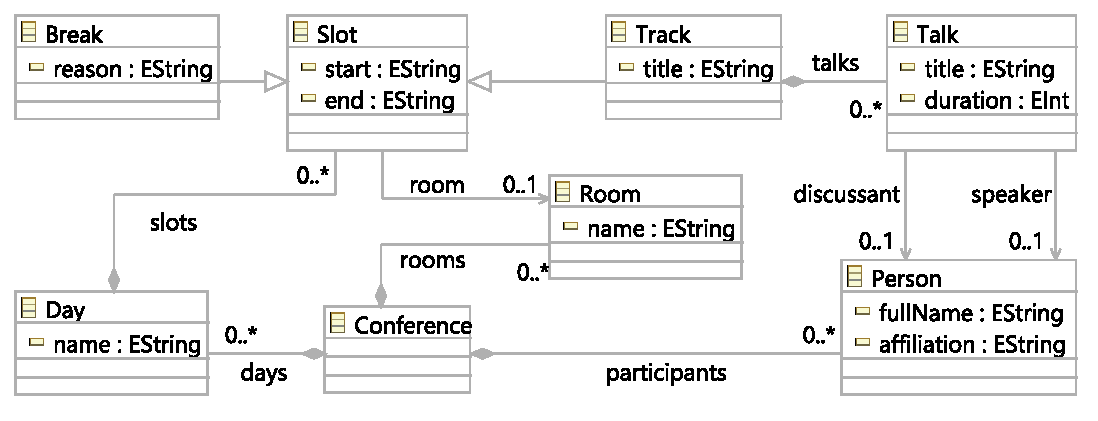
\includegraphics[width=0.9\linewidth]{conference_metamodel}
    \caption{The conference metamodel.}   
    \label{fig:node_metamodel}
\end{figure}

For our evaluation experiments, we have used synthetic models of different sizes conforming to the \emph{conference} metamodel in Fig. \ref{fig:node_metamodel}. We have selected this metamodel as it provides good coverage of the features of the EMF modelling capabilities such as single- and multi-valued features, inheritance, and containment and non-containment references. We had little option other than to use synthetic models for our experiments given that CBP is a very recent approach and we are not aware of any existing datasets containing real-world models expressed in CBP. Synthesising such models from existing state-based models (e.g. in XMI) was not an option either as state-based models do not capture editing-history-related information.    

\subsection{Loading Time}
\label{subsec:loading_time_test}

For this experiment, we created and persisted change-based models of different sizes (from 500 up to 33,000 elements) conforming to the conference metamodel of Figure \ref{fig:node_metamodel} through a random model generator that simulates the actions of a human modeller (i.e. creates/deletes elements, sets/unsets values of their features). We then used the proposed and the naive loading algorithms to reconstruct the state of these models and measured their execution time. The results are shown in Fig. \ref{fig:loading_speed_conf} and demonstrate the considerable time savings delivered by the proposed loading algorithm (it can reduce loading times up to around 44\% of the times need by the naive CBP loading algorithm for our largest models).

\begin{figure}[ht]	
    \begin{subfigure}[t]{0.5\linewidth}
		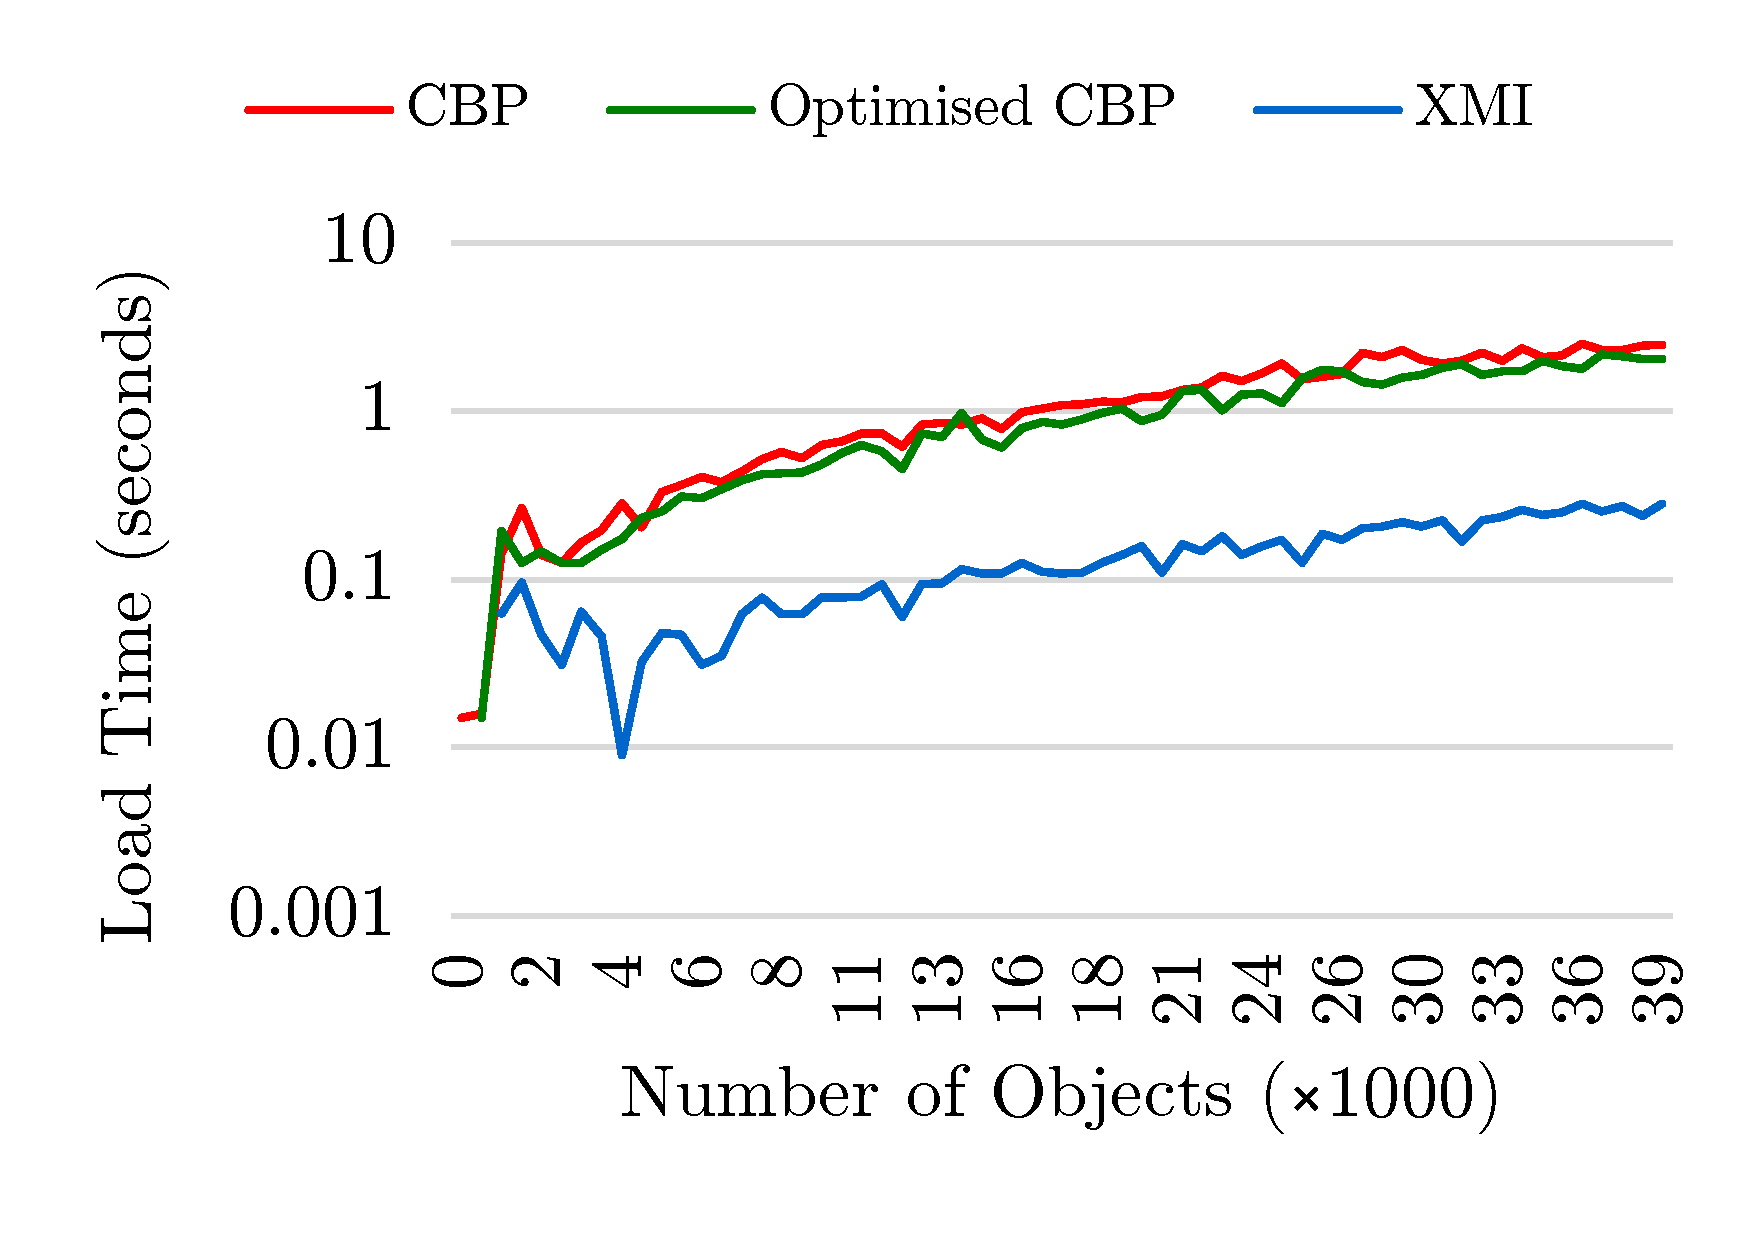
\includegraphics[width=\linewidth]{loading_speed_conf}
		\caption{Optimised CBP vs Non-optimised CBP}\label{fig:loading_speed_conf}
	\end{subfigure}
	\hfill
	\begin{subfigure}[t]{0.5\linewidth}
		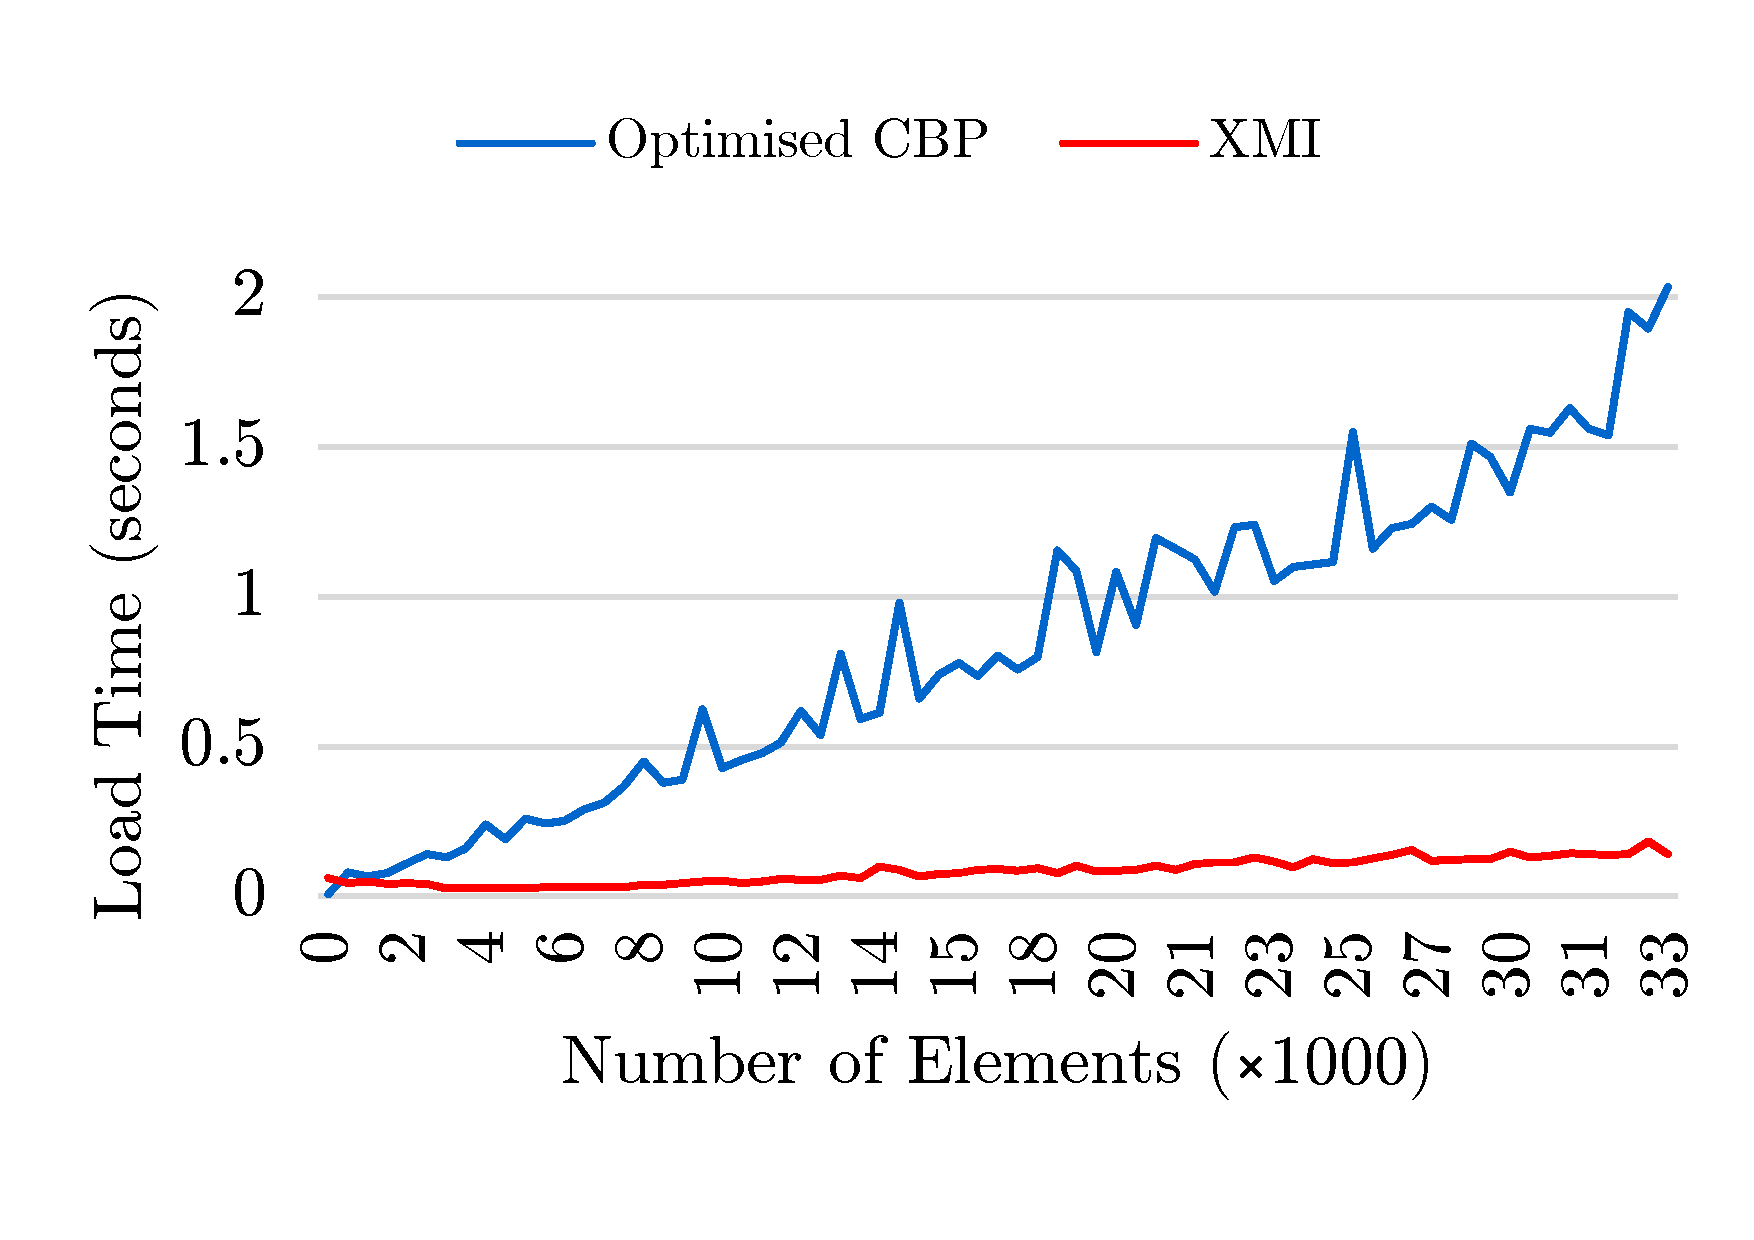
\includegraphics[width=\linewidth]{loading_speed_conf_ocbp_xmi}
		\caption{Optimised CBP vs XMI}\label{fig:loading_speed_conf_ocbp_xmi}		
	\end{subfigure}	
	\caption{A comparison on load time between optimised CBP, non-optimised CBP, and XMI.}
	\label{fig:loading_speed}
\end{figure}

For reference, we also contrast the execution time for the new algorithm against that of loading the equivalent state-based model in XMI. As can be observed in Fig. \ref{fig:loading_speed_conf_ocbp_xmi}, despite the improvements delivered by the new algorithm, loading change-based models is still roughly 10 times slower than their state-based counterparts. However, as discussed in\,\cite{yohannis2017turning}, this can be an acceptable trade-off considering the other benefits that change-based model persistence can offer (e.g. more precise differencing and hence more efficient incremental execution of model management programs and more effective model merging).

\subsection{Saving Time}
\label{subsec:saving_time_test}

To achieve the benefits in terms of loading time demonstrated in Section \ref{subsec:loading_time_test}, our algorithm requires additional work to be done (i.e. to compute and update the change Ignore List) during the model saving phase as discussed in Section \ref{sec:loading_time_optimisation}. To assess the impact of this additional work on the overall time required to save changes in models, we used a random model generator to build up multiple versions of a conference model through random sequences of creating, deleting and modifying model elements, starting with an empty model and growing it up to 22,000 elements. Every 100 new elements, the generator would save the changes and measure the time required for this activity to complete. We repeated the experiment with our prototype, with the existing baseline CBP implementation and with state-based models stored in XMI.

\begin{figure}[ht]	
    \begin{subfigure}[t]{0.5\linewidth}
		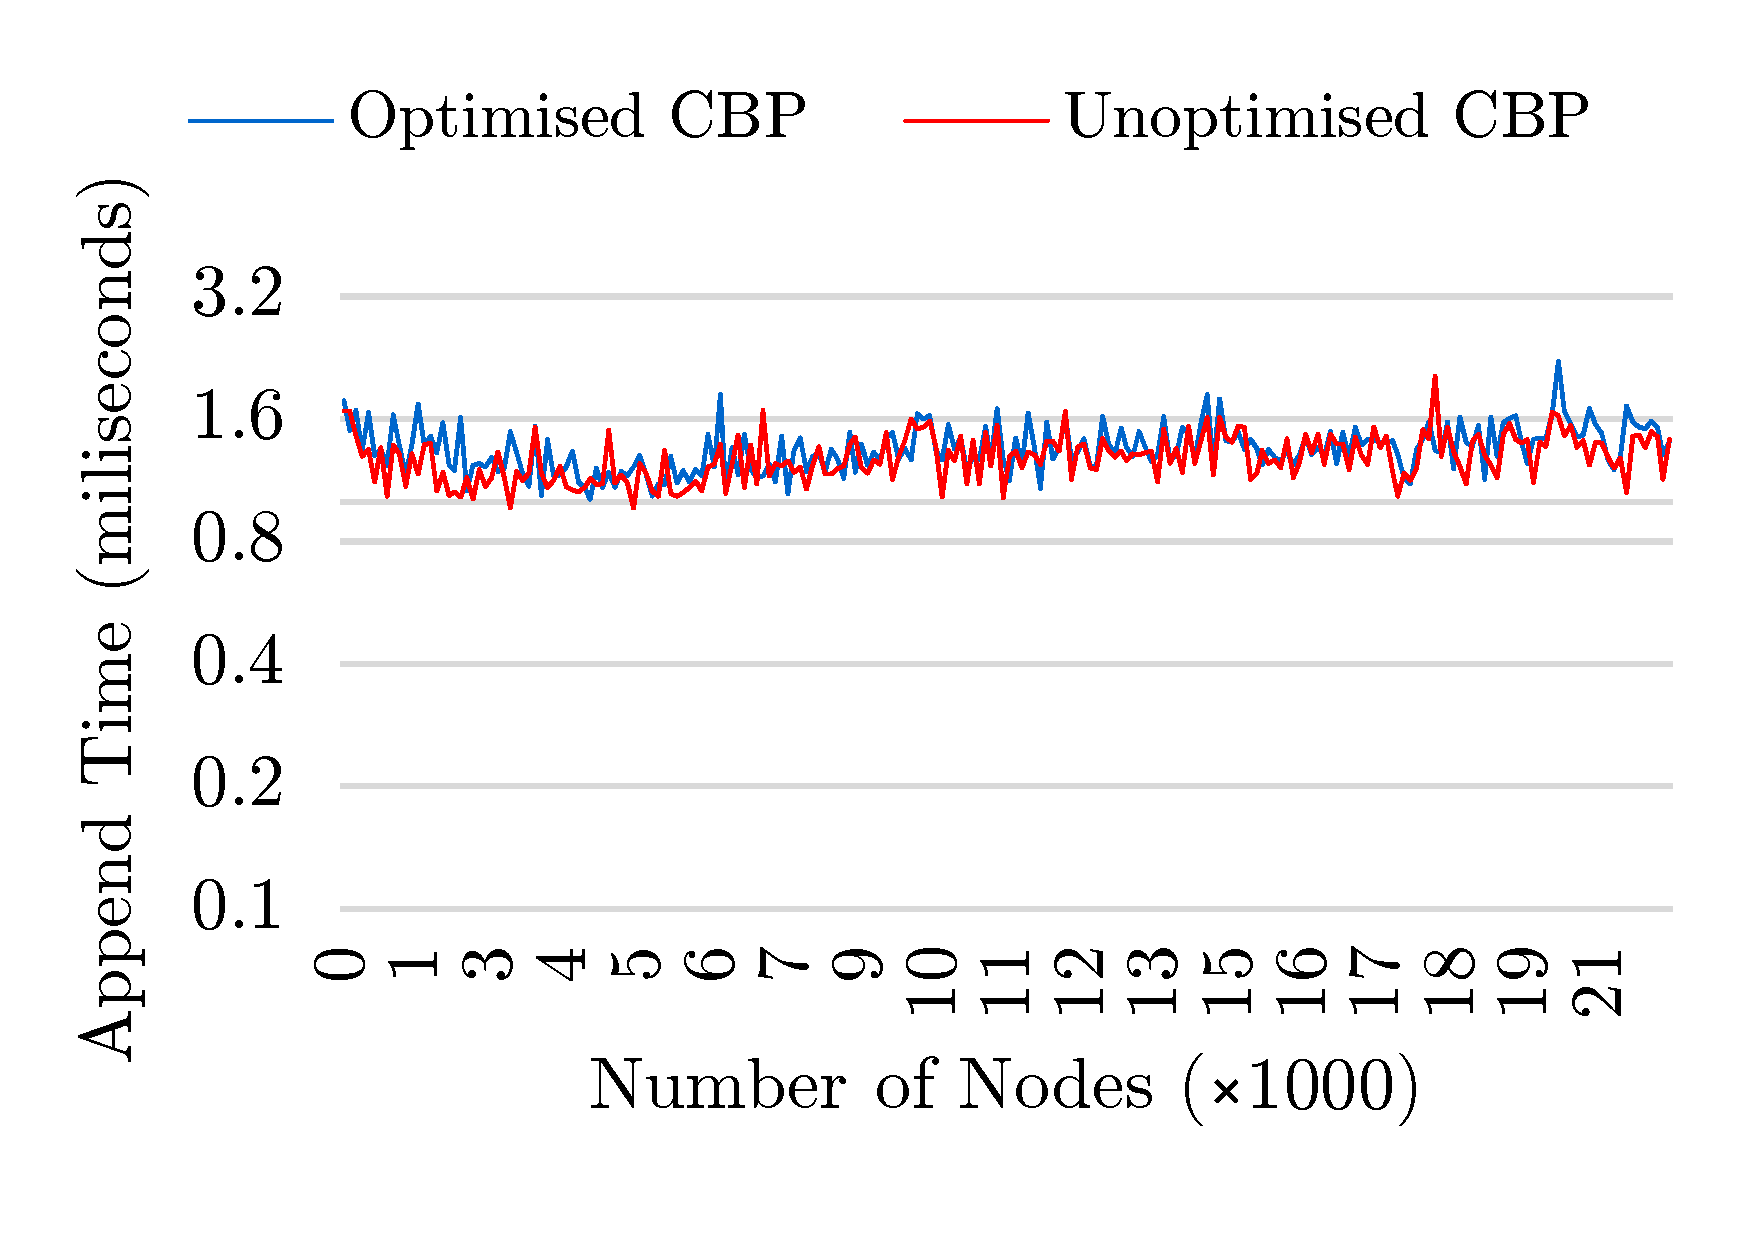
\includegraphics[width=\linewidth]{append_speed_conf}
		\caption{Optimised vs non-optimised CBPs}\label{fig:append_speed_conf}
	\end{subfigure}
	\hfill
	\begin{subfigure}[t]{0.5\linewidth}
		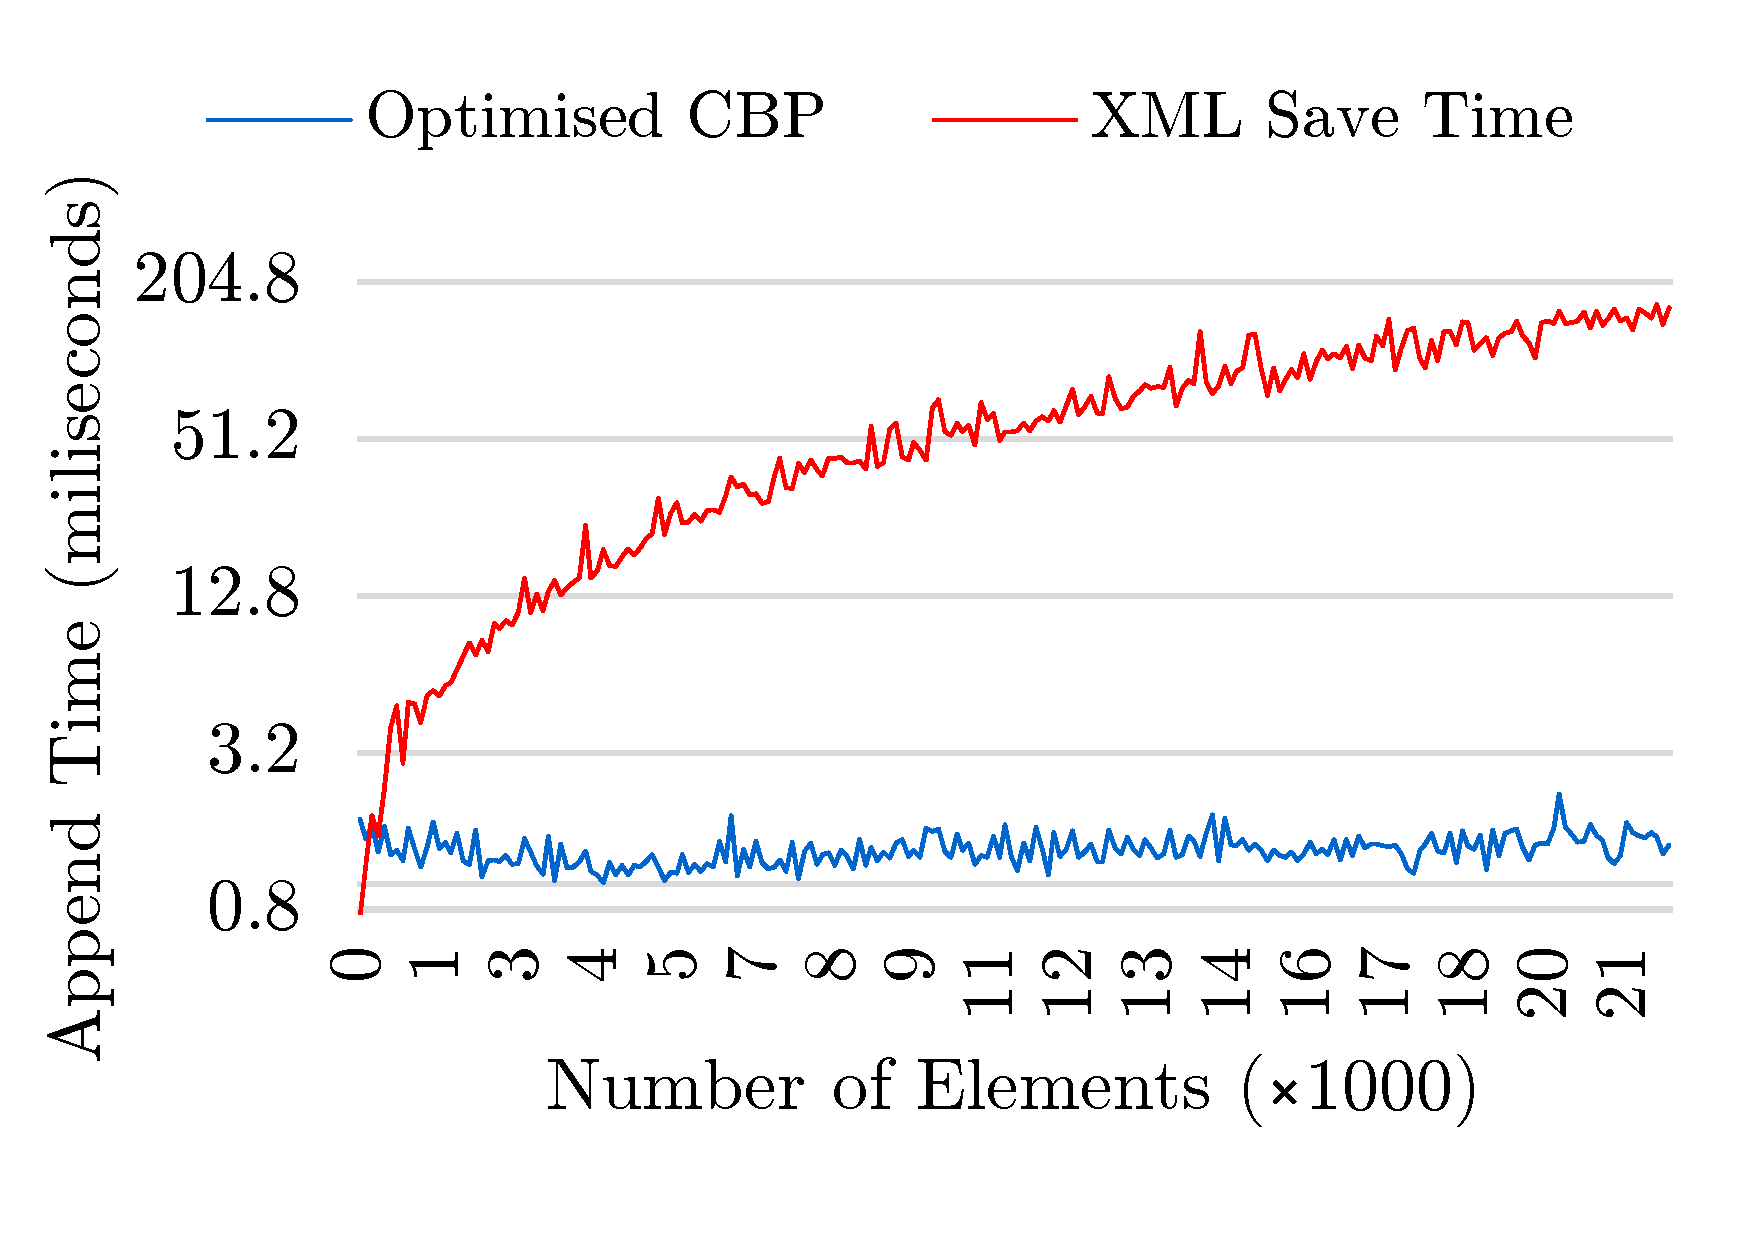
\includegraphics[width=\linewidth]{append_speed_conf_ocbp_xmi}
		\caption{Optimised CBP vs XMI}\label{fig:append_speed_conf_ocbp_xmi}		
	\end{subfigure}	
	\caption{A comparison on time used to persist models between optimised CBP, non-optimised CBP, and XMI. The y-axis is $log_2$ scaled.}
	\label{fig:append_speed}
\end{figure}

As shown in Figure \ref{fig:append_speed_conf} the performance of the two CBP implementations is almost indistinguishable, which indicates that the cost of the extra work needed by the proposed algorithm at this stage is negligible. On the other hand, CBP implementations are significantly faster at saving changes than XMI. This is expected as the CBP implementations only need to save the last batch of changes every time by appending them to the existing model file (and hence their performance is relative to the number of changes since last saved), while the XMI implementation needs to reconstruct an XML document for the entire state of the model and replace the contents of the model file every time (and hence its performance is relative to the size of the entire model). 

% We evaluate the performance of our prototype on saving time to gain insight on the efficiency that can be gained from the optimised CBP against the non-optimised CBP and XMI as the comparison baselines. The comparison is depicted in Fig. \ref{fig:append_speed}.

% We seek the relationship between number of elements in a model and the time required to persist the model. We create courses of random operations in Epsilon Object Language \cite{kolovos2006epsilon} for each tree and conference domains and executed them to simulate the development of models. In the random operations, we set the probability of different types (create, set, unset, add, move, delete) of operations to occur to 10:1:1:1:1:1 respectively. Such configuration is selected because we want the model to grow faster while other operations are still executed. Since the conference metamodel has several classes (Person, Day, Room, Break, Track, Talk), we set ratio 40:1:3:6:8:24 respectively for them to be created in the \emph{create} operation to ensure that the model is generated proportionally and closer to the the real-world conference models. We start with an empty and execute the random operations to grow the model. Along the growing of the model, we count the number of the elements. Every increase in 100 elements, we measure the time. For  the optimised and non-optimised CBPs, we measure the time consumed to append events generated for each operation, while for XMI, we measure the time used to persist the eventual state of the model after each operation. Also, we check the equivalence of the model loaded from the CBPs against its XMI format to ensure that our approach produces the correct  model.



% In Fig. \ref{fig:append_speed_conf}, the time consumed to persist events in both CBPs is nearly constant, whereas for XMI, the time consumed to persist a model increases linearly along the growth of elements (Fig. \ref{fig:append_speed_conf_ocbp_xmi}). The append time of optimised CBP is slightly higher than the non-optimised CBP's since it has to perform extra computation to populate the \emph{ModelHistory} and \emph{IgnoreList}. Based on our measurement, the average time to append in optimised and non-optimised CBPs is 1.83 and 1.33 milliseconds respectively. The average time required to save model in XMI is increased 6.22 microseconds for every additional element. This finding suggests persisting changes of a model is significantly faster than persisting its complete eventual state after the model is modified.     
         
\subsection{Memory Footprint}
\label{subsec:memory_consumption}
As the proposed loading algorithm requires the maintenance of an additional in-memory data structure that keeps track of element and feature editing histories (see Fig. \ref{fig:history_structure}), we have conducted an additional experiment to measure its memory footprint. As with the experiment in Sect. \ref{subsec:saving_time_test}, we used a random model generator to build up a conference model through random sequences of creating, deleting and modifying model elements, starting with an empty model and growing it up to 10,000 elements. Every 100 new elements, we measured the memory consumed by the program. The results are plotted in Figure \ref{fig:memory_ocbp_cbp_xmi} and demonstrate the significant overhead of the used data structure.

For reference, we also include the memory footprints of XMI in Figure \ref{fig:memory_ocbp_cbp_xmi} to contrast it with both CBP implementations. As observed, XMI outperforms the optimised CBP representation and performs slightly better than the original CBP representation on less memory footprints. 

\begin{figure}[b]	
\centering
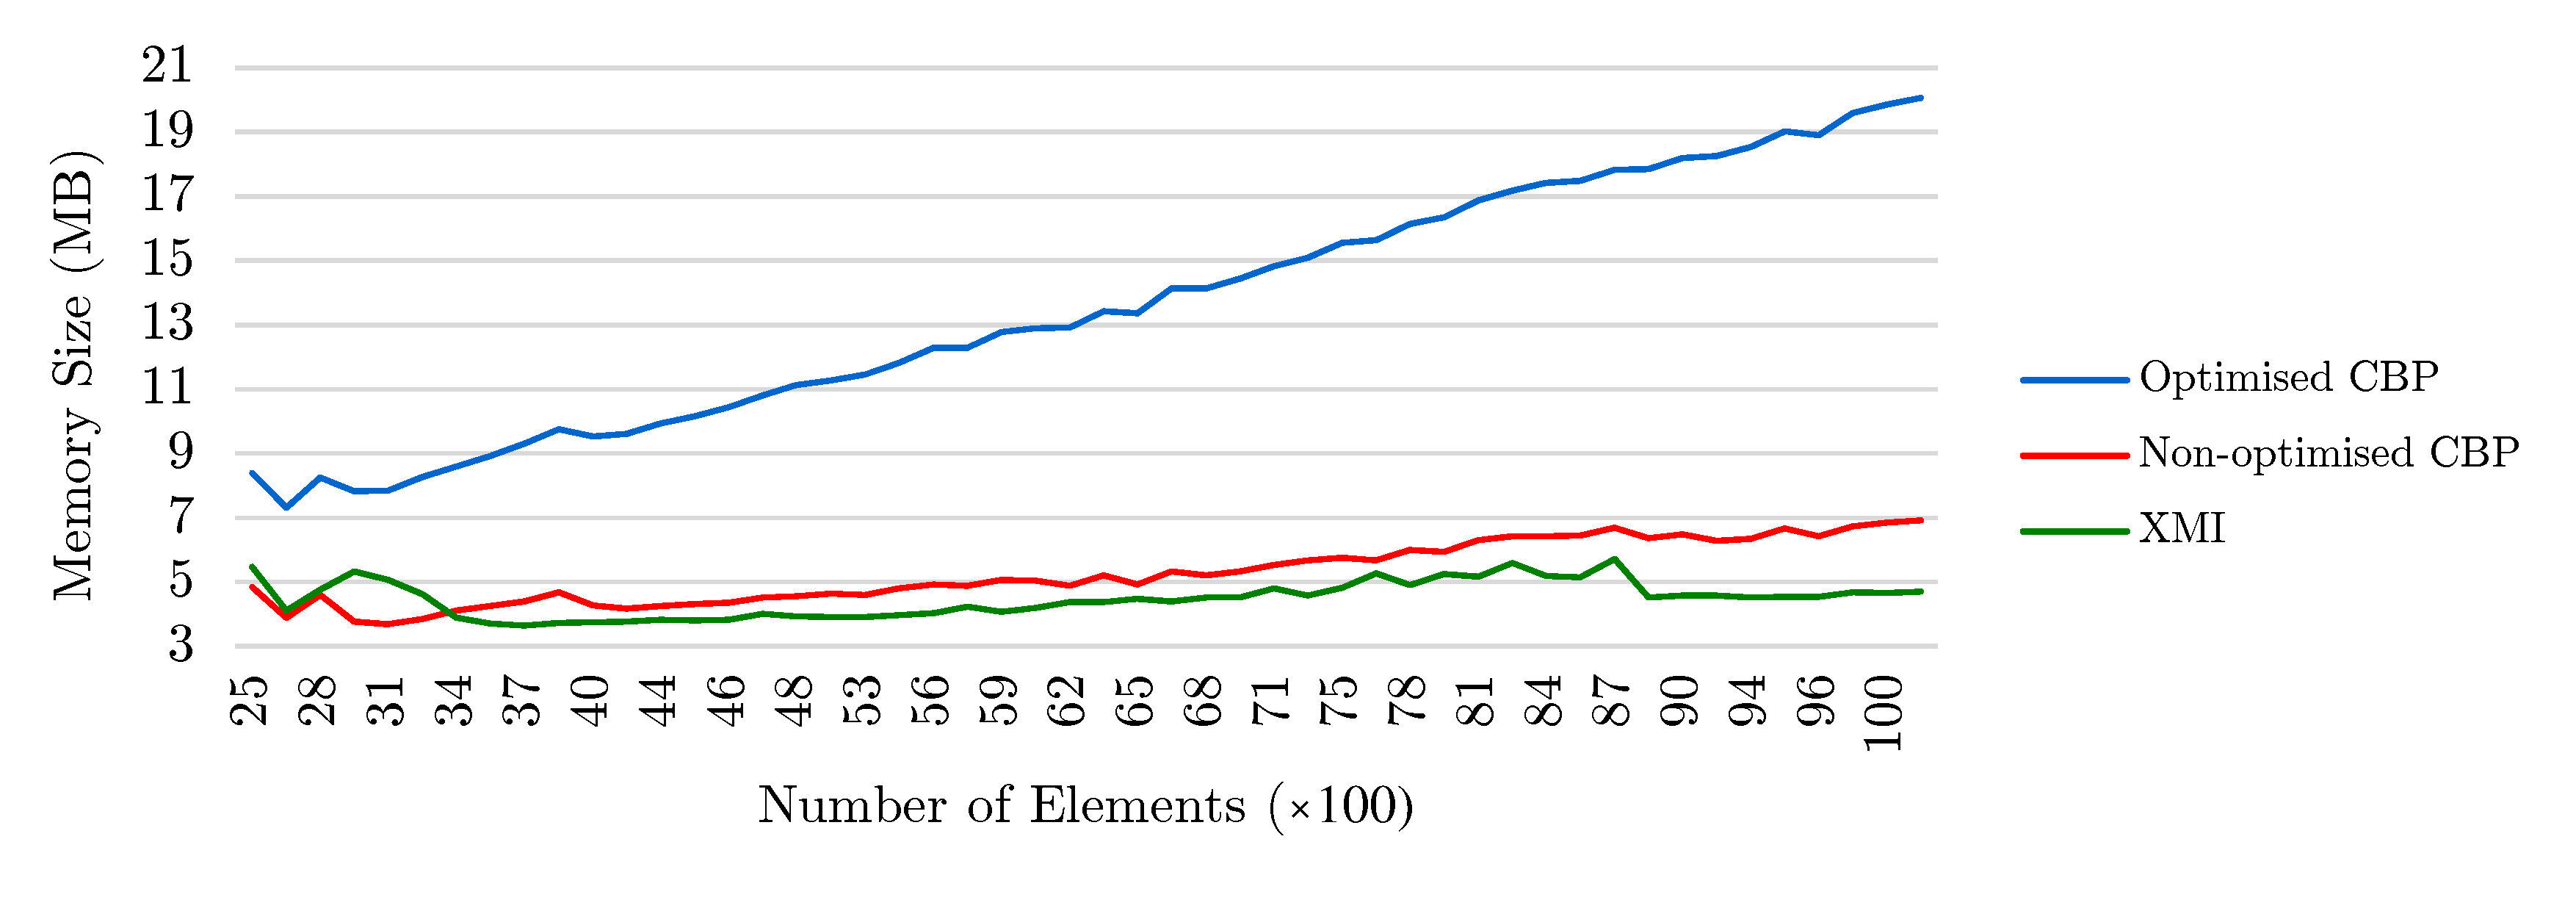
\includegraphics[width=\linewidth]{memory_ocbp_cbp_xmi}
		\caption{A comparison on memory footprints between optimised CBP, non-optimised CBP, and XMI after loading models.}\label{fig:memory_ocbp_cbp_xmi}
\end{figure}

%For reference, we also contrast the memory footprint of the CBP representation under the new algorithm against that of XMI. As observed in Figure \ref{fig:memory_ocbp_cbp_xmi}, 

%TODO: Discuss threats to the validity/generalisability of these findings e.g. using synthesised models, not running the experiments in multiple iterations etc.

% We also compare optimised CBP, non-optimised CBP, and XMI on their memory consumption after loading models. We seek the relationship between number of elements of a model and memory used to after loading the model. The results are shown in Figure \ref{fig:memory_use}. In performing the simulation, we performed the same procedure as in the loading time evaluation (subsection \ref{subsec:loading_time_test}), except for the increment and the dimension that we measure. We set the increment to 100, and instead of measuring the loading time, we measure the memory consumption by subtracting the memory after loading a model with the memory before loading the model.   

% Figure \ref{fig:memory_use_conf_ocbp_xmi} shows that optimised CBP consumes more memory than non-optimised CBP, while XMI performs a slightly better than non-optimised CBP in terms of memory saving (Fig. \ref{fig:memory_use_conf_cbp_xmi}). The large memory consumption of optimised CBP is caused by the Ignore List which is used for checking events in a CBP if they can be ignored for replay or not. %This condition leads us to another future work that is to identify and remove elements, events, and events numbers from the Model History once they are not any longer required. For example, once a element is deleted from a model, all its records in the Model History are removed to release space in memory. 

%\begin{figure}[ht]	
%	\begin{subfigure}[t]{0.5\linewidth}
%		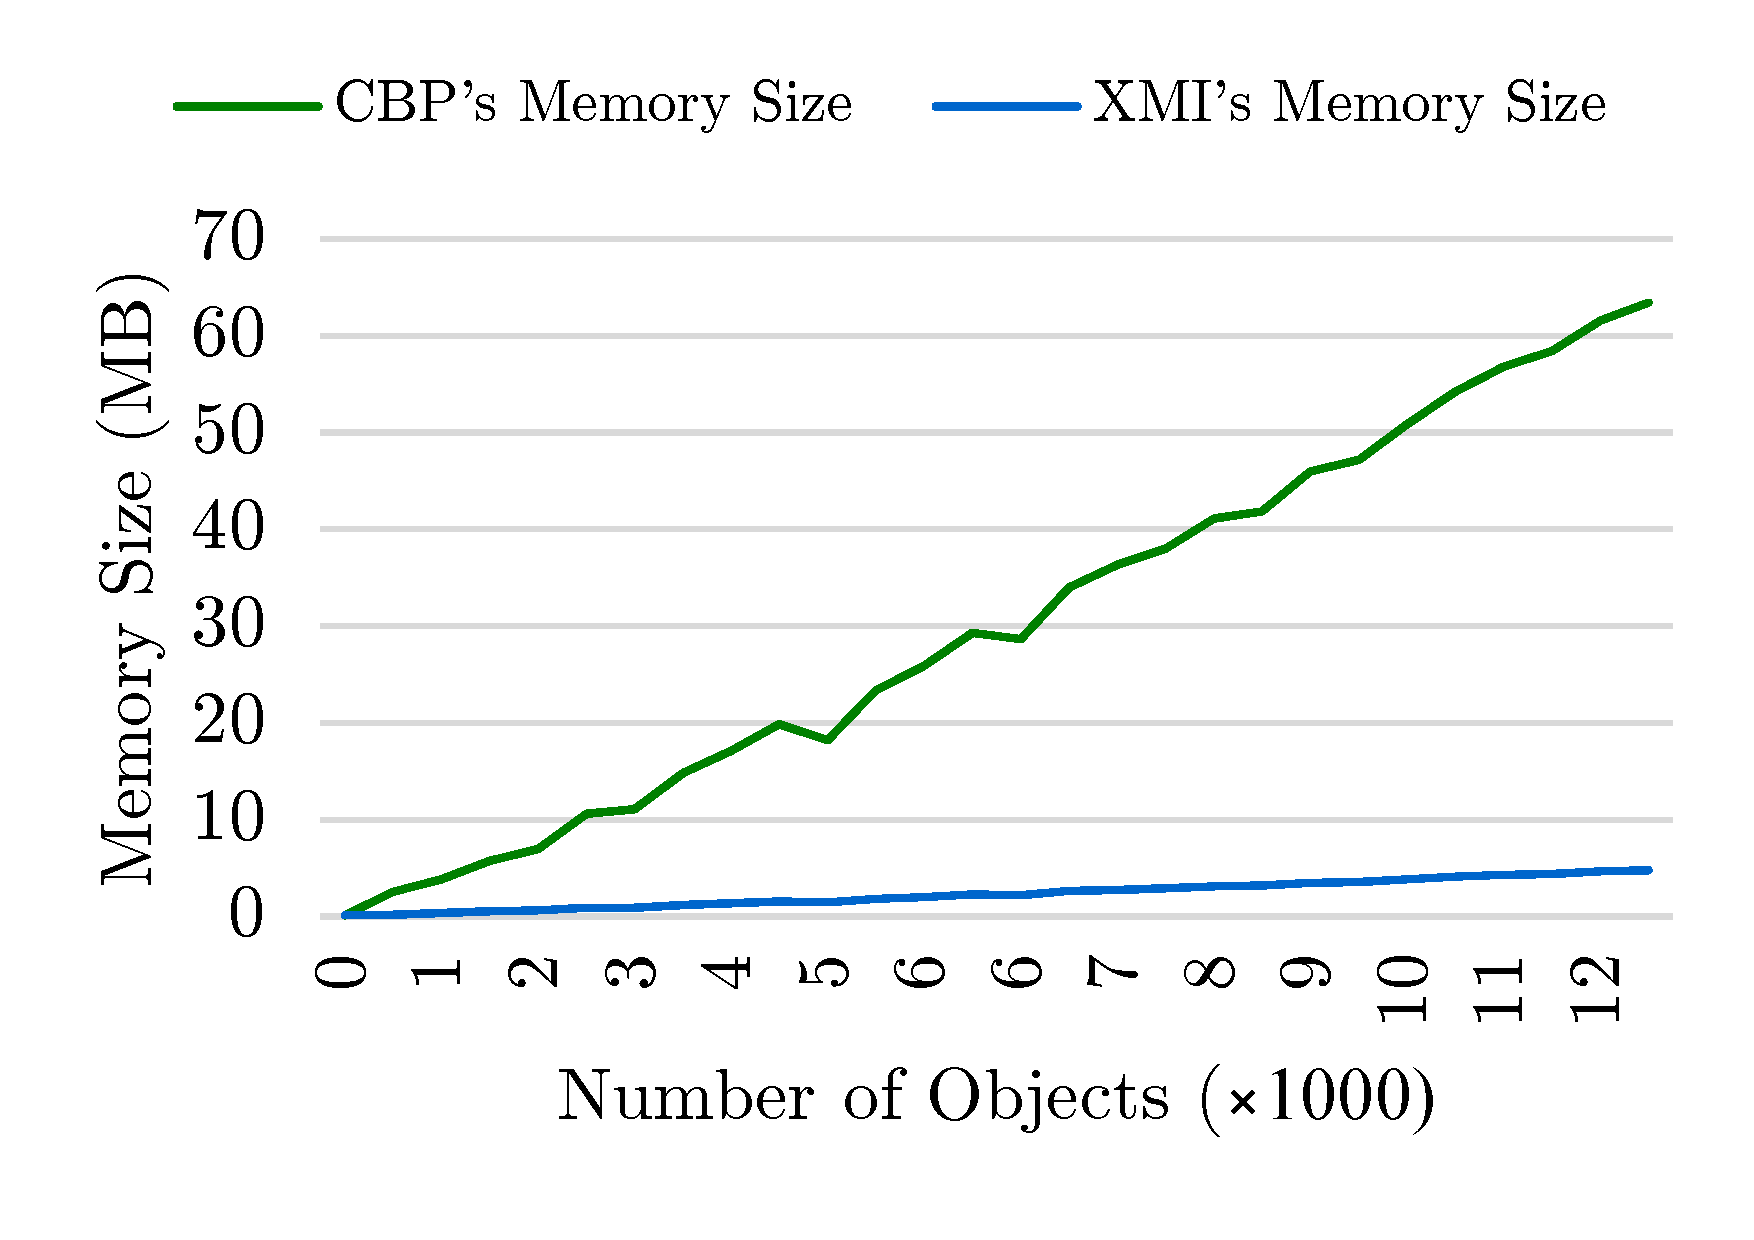
\includegraphics[width=\linewidth]{memory_use_conf}
%		\caption{Optimised vs non-optimised CBPs}\label{fig:memory_use_conf_ocbp_xmi}		
%	\end{subfigure}
%	\hfill
%	\begin{subfigure}[t]{0.5\linewidth}
%		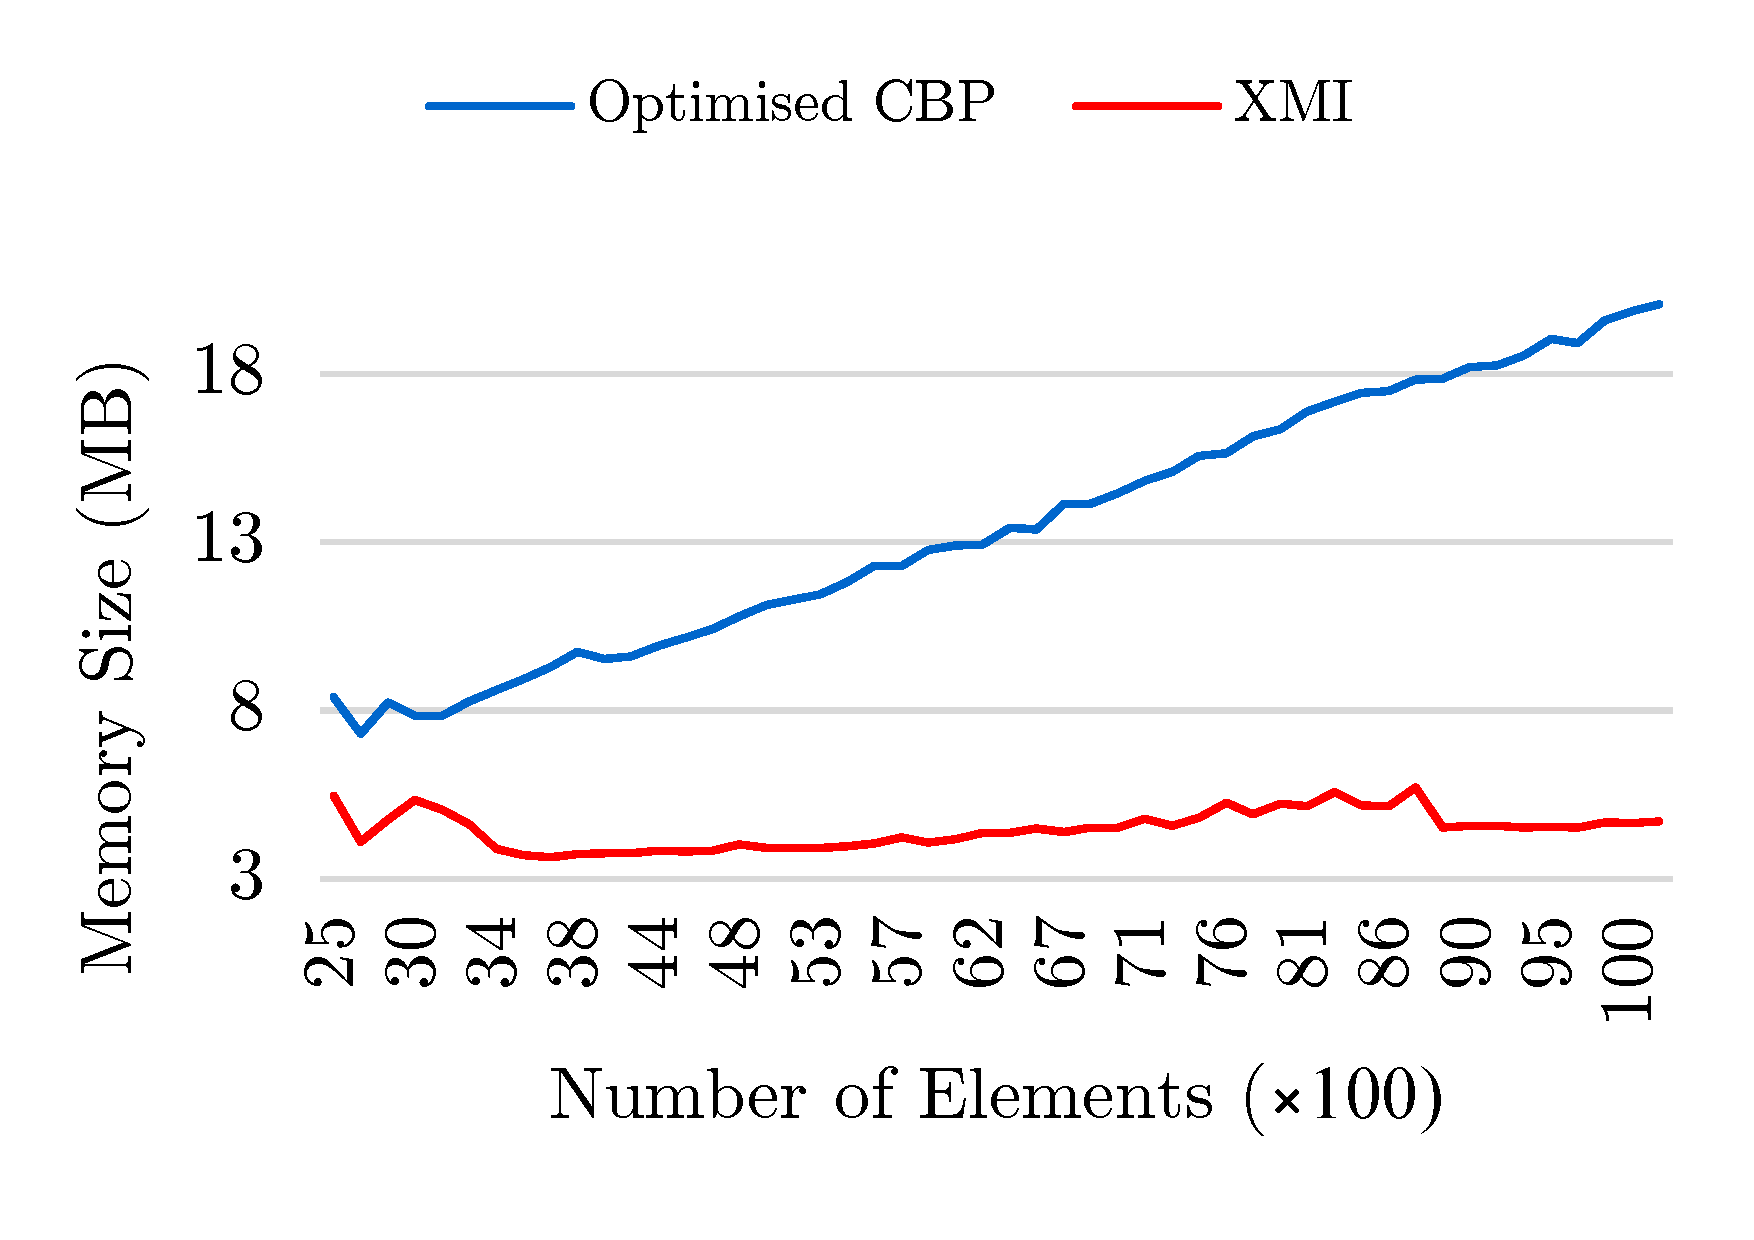
\includegraphics[width=\linewidth]{memory_use_conf_cbp_xmi}
%		\caption{Non-optimised CBP vs XMI}\label{fig:memory_use_conf_cbp_xmi}
%	\end{subfigure}
%	\caption{Memory consumption of optimised CBP, non-optimised CBP, and XMI.}
%	\label{fig:memory_use}
%\end{figure}

\subsection{Threats to Validity and Limitations}
\label{sec:limitations_and_future_work}
In this work, we have only tested the algorithm on synthesised conference models which do not perfectly represent real-world models. Diverse characteristics of models in different domains can affect the effectiveness of the algorithm and therefore yields different outcomes. Also, we have not run the experiments on multiple iterations to obtain more consistent and stable results. Moreover, we have not performed the experiments on different types of environments (e.g. machines, operating systems, Java versions, modelling frameworks). Different environments might affect the experiments to produce different results. 

We only address feature that can only contain ordered, unique members -- no duplicate values or elements.
The `duplicate members' means that removal of a member does not result in the member not being present in the feature value.
Additional information must be captured during insertion to persist the number of copies and positions of the feature members.
In the algorithms, this information can be used to properly generate the Ignore List.
In the case of unordered features, the moved event does not exist, and hence analysis will be required to determine how this affects the use of the \emph{featureIsMoved} flag. 

Given that it is impossible to generalise a metamodel structure and as such, the examples used in this work will only represent a subset of the possible/existing metamodels. As a result, we expect different metamodels to exhibit different gains when using the optimized CBP. Moreover, our prototype still consumes a significant amount of memory in executing the algorithm and still performs more than 10 times slower than XMI in loading models. Thus, we have identified several approaches to improve more of the performance in section \ref{sec:conclusions}.

\section{Related Work}
\label{sec:related_work}
Several works have investigated alternative model persistence mechanisms to XMI, mainly by using databases (both relational and NoSQL). Connected Data Objects \cite{eclipse2017cdo} and EMF Teneo\,\cite{eclipse2017teneo} persist EMF models in relational databases.
Both approaches use the metamodel to generate the database schema and provide a high-level abstraction API for developers to seamlessly interact with the databases. The main drawback of using relational databases is that highly interconnected models result in expensive joins over multiple tables \cite{barmpis2014evaluation}. 

Morsa \cite{pagan2011morsa} and NeoEMF \cite{daniel2016neoemf} persist models in NoSQL databases.
Morsa uses MongoDB\,\cite{mongodb2017what} to persist models as a collection of documents by storing every element of a model (and its metamodel) as entries in an index document that refer to the root elements of the model's elements' documents.%No comprendo!!
However, due to the nature of document-based databases, storing model element references as serialised documents limits their querying and insertion performance\,\cite{barmpis2014evaluation}.
NeoEMF can persist models in different NoSQL databases and provides a lazy-loading mechanism to improve accessing, loading, and removing model elements. Extending NeoEMF to support distributed collaborative modelling is still an ongoing work \cite{sunye2017model}.
%Nevertheless, it has not addressed the issues of collaboration, versioning,
%\dk{This is not accurate. CDO supports both collaboration and versioning}
%and fast model differencing.

EMFStore\,\cite{koegel2010emfstore} is a version control system (VCS) that stores changes of models as operations applied to the models, which facilitates collaboration and identify changes of models easier.
However, support to use its operation-based approach with more common VCSs (e.g. GitHub, SVN) is not yet available. Several papers mention it does not scale\,\cite{pagan2011morsa,kolovos2013research} and no optimisation has been proposed to load the eventual versions of models, except replaying all stored operations. 

\section{Conclusions and Future Work}
\label{sec:conclusions}
In this paper, we have proposed an optimization to the CBP model in order to improve its performance, in particular to the loading time.
We evaluated our approach against the original CBP model and the de-facto XMI persistence, on loading but also on store time and memory consumption of the loading process. 
Our results show considerable savings in terms of store times and identifying changes made to models at an increased -- but linear -- model loading cost. 

For future work, we plan to perform experiments in which modellers are asked to construct complex models using different modelling languages, persist their histories, scale them up, simulate the loading optimisation, and analyse the results to gain insight whether the optimisation really works for real-world models. 
A number of approaches also has been identified to reduce the memory consumption and loading time.
Possible areas of interest are:
Optimising the format of CBP so that it consumes less memory and can be parsed faster.
Persisting all events into databases therefore can reduce the use of main memory, and NoSQL databases can be considered to improve the loading performance.
Develop a hybrid persistence representation that is a combination of state-based and change-based persistence.
Finally, given that NeoEMF can handle large-scale models, we plan to extend it to support change-based persistence.
Moreover, we also plan to extend the CBP to enable change detection, model merging, conflict resolution of models in the context of collaborative modelling, among others. 
Accommodating the evolution of metamodel into change-based persistence is also an interesting challenge to investigate.

%\subsubsection*{Acknowledgments.} This work was partly supported through a scholarship managed by \emph{Lembaga Pengelola Dana Pendidikan Indonesia} (Indonesia Endowment Fund for Education).

\bibliography{references} 
\bibliographystyle{splncs}

\end{document}
